\documentclass{ieeeaccess}
\usepackage{cite}
\usepackage{amsmath,amssymb,amsfonts}
\usepackage{algorithmic}
\usepackage{textcomp}
\usepackage{bm}
\usepackage{multirow}
\usepackage{tabu}
\usepackage{mathtools}
\usepackage{subcaption}
\usepackage{caption}
\usepackage{nicefrac}
\DeclarePairedDelimiter{\abs}{\lvert}{\rvert}
\usepackage[inline]{enumitem}
\usepackage[nopostdot,nonumberlist]{glossaries}
\renewcommand{\baselinestretch}{1.000}
% *** GRAPHICS RELATED PACKAGES ***
%
\ifCLASSINFOpdf
\usepackage[pdftex]{graphicx}
% declare the path(s) where your graphic files are
\graphicspath{{../images/}}
% and their extensions so you won't have to specify these with
% every instance of \includegraphics
\DeclareGraphicsExtensions{.pdf,.jpeg,.jpg,.png}
\else
% or other class option (dvipsone, dvipdf, if not using dvips). graphicx
% will default to the driver specified in the system graphics.cfg if no
% driver is specified.
\usepackage[dvips]{graphicx}
% declare the path(s) where your graphic files are
\graphicspath{{../eps/}}
% and their extensions so you won't have to specify these with
% every instance of \includegraphics
\DeclareGraphicsExtensions{.eps}
\fi

\def\BibTeX{{\rm B\kern-.05em{\sc i\kern-.025em b}\kern-.08em
    T\kern-.1667em\lower.7ex\hbox{E}\kern-.125emX}}

% place the makeglossary at the preamble
%\newglossary[nlg]{notation}{not}{ntn}{List of Symbols and Acronyms}


% type out the glossaries
\newacronym{zlabel}{$ \bm{\vec{z}} $}{latent input sample to generator}
\newacronym{clabel}{$\bm{\vec{c}} $}{conditional input sample}
\newacronym{genuoutput}{$ \bm{\vec{y}_{g}}$}{generator output}
\newacronym{noiseinput}{$ \bm{\widetilde{x}} $}{additive synthetic noise input}
\newacronym{genericdiscinput}{$ \bm{\vec{y}} $}{discriminator input}
\newacronym{realsamples}{$ \bm{\vec{x}_d} $}{real sample input to the discriminator}
\newacronym{discoutput}{$ \bm{\vec{y}_{d}} $}{discriminator output}
\newacronym{discfunction}{$ \bm{D} $}{discriminator transformative function}
\newacronym{genfunction}{$ \bm{G} $}{generator transformative function}
\newacronym{discloss}{$ \bm{L_D} $}{discriminator loss}
\newacronym{genloss}{$ \bm{L_G} $}{generator loss}
\newacronym{gsingle}{$ \bm{G_s} $}{single class GAN generator}
\newacronym{gbinary}{$ \bm{G_b} $}{binary class GAN generator}
\newacronym{tsne}{$ \bm{P_{j|i}} $}{probability of point $ j $ choosing $ i $ as a neighbor}
\newacronym{distance}{$ \bm{C}_i $}{cluster $ \bm{i} $ for $ \bm{i  \in  \{0,1\}} $ }
\newacronym{centroids}{$ \bm{\left(\bar{m}_i,\bar{n}_i\right)} $}{centroid cordinates of the detector for $ \bm{i  \in  \{0,1\}} $ }
\newacronym{tsneoutput}{$ \bm{(m_j,n_j)} $}{embedding output tuple of sample $ \bm{j} $}
\newacronym{norm}{$ \bm{p_{2_i}} $}{euclidean norm to a cluster $ \bm{i} $}

\makeglossaries	


\begin{document}

\history{Date of publication xxxx 00, 0000, date of current version xxxx 00, 0000.}
\doi{10.1109/ACCESS.2020.DOI}

\title{AD-CGAN: Anomaly Detection using Conditional Generative Adversarial Networks}
\author{\uppercase{Okwudili M. Ezeme}, \IEEEmembership{Member, IEEE},
\uppercase{Qusay H. Mahmoud, \IEEEmembership{Senior Member, IEEE} and Akramul Azim \IEEEmembership{Senior Member, IEEE}}}
\address{Department of Electrical, Computer and Software Engineering \\
	Ontario Tech University, Oshawa, ON L1G 0C5 Canada\\
	(e-mail: \{mellitus.ezeme, qusay.mahmoud, akramul.azim\}@ontariotechu.net)}
%\tfootnote{This research was funded in part by the Natural Sciences and Engineering Research Council of Canada (NSERC).}

\markboth
{Ezeme, O. \headeretal: AD-CGAN: Anomaly Detection using CGAN}
{Ezeme, O. \headeretal: AD-CGAN: Anomaly Detection using CGAN}

\corresp{Corresponding author: Okwudili Ezeme (e-mail: mellitus.ezeme@ontariotechu.net).}

\begin{abstract}
Whether in the realm of software or hardware, datasets that represent the state of systems are mostly imbalanced. This imbalance is because the reliability requirements of these systems make the occurrence of an anomaly a rare phenomenon. Hence, most datasets on anomaly detection have a relatively small percentage that captures the anomaly. Recently, generative adversarial networks (GAN) have shown promising results in image generation tasks. Therefore, in this research work, we build on the ability of conditional GANs (CGAN) to generate plausible distributions of a given profile to solve the challenge of data imbalance in anomaly detection tasks and present a novel framework for anomaly detection. Firstly, we learn the pattern of the minority class data samples using a \textit{single class CGAN}. Secondly, we use the knowledge base of the single class CGAN to generate samples that augment the minority class samples so that \textit{a binary class CGAN} can train on the typical and malicious profiles with a balanced dataset. This approach inherently eliminates the bias imposed on algorithms from the dataset and results in a robust framework with improved generalization. Thirdly, the binary class CGAN generates a knowledge base that we use to construct the cluster-based anomaly detector. During testing,  we do not use the single class CGAN, thereby providing us with a lean and efficient algorithm for anomaly detection that can do anomaly detection on semi-supervised and non-parametric multivariate data. 
We test the framework on logs and image-based anomaly detection datasets with class imbalance.
We compare the performance of AD-CGAN with similar cluster-based algorithms that have been tested on the same benchmark datasets, and AD-CGAN outperforms all the other algorithms in the standard metrics for measuring the efficacy of anomaly detection algorithms.
\end{abstract}

\begin{keywords}
Anomaly Detection, Transfer Learning, Deep Learning, Generative Adversarial Networks
\end{keywords}

\titlepgskip=-15pt

\maketitle
\section{Introduction}
\label{sec:introduction}
In data mining and statistics, an outlier or anomaly refers to the characteristics of being different from others considered normal, and the field of \emph{anomaly detection} is concerned with the detection of these deviants using a well defined statistical or machine learning procedure\cite{wang2019progress,yuansurveyacmanom}. According to \cite{hawkins1980identification}, an anomaly differs from other samples by having features which suggest that the process that generated the anomalous sample is different from the process that generated the rest of the samples. Also, the presence of anomalies can be as a result of errors in software that generates the data, problems with the data collection methods or an outright attack on the application by agents that try to take control of the application. Therefore, an anomaly can be \textit{point-based, radius-based} or \textit{context-based} \cite{liu2012isolation}.
With the increasing integration of machine learning and deep learning frameworks into so many areas of computing and business intelligence, the anomaly detection practitioners still rely heavily on the use of signature-based anomaly detection mechanism because most of them trade \textit{determinism} for \textit{generalization}. However, deep learning based models offer the following advantages over the traditional algorithms \cite{bahnsen_2017,chalapathy2019deep}:
\begin{enumerate*}[label={\alph*)},font={\bfseries}]
	\item they scale better when the dataset is large, and because we are in the big data age, deep learning networks seem appropriate for anomaly detection especially in the online deviant behavior detection;
	\item there is no need for feature engineering by domain experts since the cascade of layers in the deep learning frameworks does automatic feature processing, thereby providing an end-to-end model that takes raw data and returns a decision;
	\item deep learning models have outperformed traditional algorithms in processing time-series and image data.
\end{enumerate*}
Despite all these advantages, the adoption of these deep learning models in anomaly detection is still not wide-spread because the evolving nature of the boundary between normal and deviant behaviors in several domains makes it difficult to demarcate with certainty, the anomalous and normal data from each other. Hence, the prevalence of the signature-based approaches despite the advantage of detecting zero-day vulnerabilities with anomaly models. Furthermore, considering that investigation and confirmation of an alarm to be a false alarm requires enormous resources both in terms of human and material capital, some companies often trade the risk of exploitation of zero-day vulnerabilities to committing resources into the investigation of false alarms. Some others use a combination of both the signature and model-based approaches depending on the criticality of the resource being protected and the financial outlay of the company.  
Recently, GANs \cite{goodfellow2014generative} have emerged as an important area of deep learning with ground breaking results in mostly image, audio and video applications. There are different variants of GAN \cite{wang2019generative} and we build on \cite{mirza2014conditional} to design our AD-CGAN used for anomaly detection in imbalanced data. Since GANs draw samples from the latent space, this research has the ability to provide a more stable prediction since it does not suffer from cumulative errors that are inherent in linear models like the autoregressive integrated moving average (ARIMA) \cite{zhang2003time}.
 
%\printglossaries

\subsection{Motivations and Contributions}
\label{subsec:time-event}
Applications and cyber-physical systems are designed with high-reliability requirements. Therefore, most of the time, the data collected from these systems contains normal operating conditions and some occasional anomalous incidents. Because of the rarity of occurrence of these unusual incidents, many datasets used by researchers to model system profiles in this domain are highly imbalanced, resulting in the following consequences: 
\begin{enumerate}[label={\alph*)},font={\bfseries}]
	\item bias is inherently introduced in the models built using the imbalanced data. Since random guess is guaranteed to return high accuracy due to the data imbalance, machine learning models appear redundant.
	\item adaptability of anomaly detection frameworks from one system to another with varying ratios of typical to anomalous samples returns poor performance because bias varies from one system to the other. This variability in the composition of the different datasets makes generalization difficult.
\end{enumerate}
Therefore, our contributions in this research work are as follows;
\begin{enumerate}[label={\alph*)},font={\bfseries}]
    \item design and development of a CGAN for context modeling of \textit{normal} and \textit{malicious} profiles.
	\item creation of a multi-stage transfer learning framework using \textit{CGANs} to generate distinct clusters in imbalanced data. 
	\item introduction of a lightweight anomaly detector for anomaly detection in non-parametric multivariate data using the knowledge base of the CGANs.
\end{enumerate}
We organize the rest of the paper into the following sections: Section \ref{sec:related-work} highlights some of the related works in this domain while Section \ref{sec:design} discusses the details of the AD-CGAN design. In Section \ref{sec:experiments}, we conduct experiments on benchmark datasets to measure the performance of AD-CGAN and discuss the results of the experiments in Section \ref{sec:results}. Finally, we conclude the paper in Section \ref{sec:conclusion} and offer ideas for future work.
\section{Related Work}
\label{sec:related-work}
\textit{Intrusion} and \textit{anomaly} detection \cite{chandola2009anomaly,mutz2006anomalous,yuansurveyacmanom} are the two broad classifications of detecting deviant behaviors in a system or application. While 
intrusion detection techniques rely on the use of \emph{signatures} to detect a 
misuse behavior by storing signatures of discovered anomalies, anomaly 
detection models construct contexts using known standard features, and labels 
any deviation from the constructed profile as anomalous. The obvious limitation 
of this signature-based approach is that \emph{zero-day} vulnerabilities cannot 
be detected as it only searches for observed signatures, i.e. \emph{it 
	emphasizes memorization over generalization}. On the other hand, the 
anomaly-based approaches target both known and unknown anomalies and can 
detect \emph{zero-day} vulnerability. Because our work centers on anomaly 
detection approach, we highlight mostly the works in this area. \par 
In \cite{ezeme2017imputation,ezeme2020peskea}, the authors used kernel events to build an offline anomaly 
detection model using some vector space model concepts and agglomerative 
clustering technique. Imputation techniques were also used to increase the 
scope of their model and reduce the incidents of false 
positives. However, the anomaly frameworks of \cite{ezeme2017imputation,ezeme2020peskea} lack temporal modeling, hence, does not capture the nature of the system process behavior which emits system calls in discrete, sequential mode. Reference \cite{du2017deeplog} used deep LSTM models constructed 
from system logs to create anomaly detection models for detecting anomalies in logs from virtual machines. The LSTM model is 
augmented with a workflow model which helps to detect context switches but since it is a host-based anomaly framework, it lacks the fine granularity of process-based anomaly detection frameworks. Authors 
of \cite{xu2009largescale} used textual information buried in console logs 
of a program to create an anomaly detection model 
using principal component analysis that analyzes user credentials and actions. Also, \cite{mutz2006anomalous} constructed 
host-based anomaly detection models using Bayesian Networks that uses system 
call arguments and variables as its features. The model of 
\cite{mutz2006anomalous} uses aggregate weighting to reduce the effect of 
inconsistent anomaly scores from different models, but they do not consider the 
temporal relationship amongst the sequence of the system calls. Also, in 
\cite{EzemeHaBAD,ezeme2019dream}, the hierarchical LSTM network is used to explore 
the 
understanding of relationships amongst the kernel event traces of an embedded 
system, but other features which ordinarily should yield a more representative 
model like timestamps, CPU cycles, and system call arguments are skipped.
\par 
Authors of \cite{yoon2017learning} have an anomaly model built using system 
call frequency distribution as well as clustering techniques to detect when 
processes deviate from their standard profiles. Similar to the anomaly frameworks of \cite{ezeme2017imputation,ezeme2020peskea}, the model of \cite{yoon2017learning} has no temporal modeling of the events and can only be used for post-mortem analysis. Furthermore, the authors of 
\cite{gu2005detecting} used the statistical metric of entropy to implement an 
anomaly detection model for network logs, but this type of anomaly model is 
best suited for cases where the volume of logs determine if an anomaly has 
occurred as obtainable in denial of service attacks. Also, the model of 
\cite{gu2005detecting}'s use of entropy as the discriminating factor makes the 
result non-specific as entropy values are not unique. In 
\cite{salem2016anomaly}, a real-time systems anomaly detection model is 
designed using the principle of inter-arrival curves to detect anomalous traces 
in a log sequence. Again, this inter-arrival curve-based model ignores 
other properties of system calls and is suitable for offline analysis only. The authors of \cite{li2017locating} used an 
optimization method of minimum debugging frontier sets to create a model for 
detection of errors/faults in software execution. Also, 
\cite{kosoresow1997intrusion} used 
system call traces without arguments to create an anomalous profile detector 
using deterministic finite automaton (DFA). The authors assume that anomalous 
system call sequences have a local profile and that with the use of a 
\emph{locality frame}, these anomalies can be detected. And this \emph{local profile} assumption is the limitation of the work as sophistication in cyber attacks has shown that both local and non-local profiles are exploited in the design of anomalies. Authors of 
\cite{kosoresow1997intrusion} however admitted that when the anomalous 
sequences are not concentrated in a burst; their algorithm cannot handle such 
scenarios. Reference \cite{warrender1999detecting} used techniques such as the 
\emph{counting of observed system calls, frequency distribution approaches, a 
	rule-based technique called RIPPER and a Hidden Markov Model (HMM)} to 
construct anomaly models to detect valid and irregular behavioral profiles. 
Furthermore, in \cite{hofmeyr1998intrusion}, a sliding window approach is used to 
construct a tree of the possible routes of the system call sequences based on 
the observed behavior during the learning phase.
\begin{figure}[h!]
	\centering
	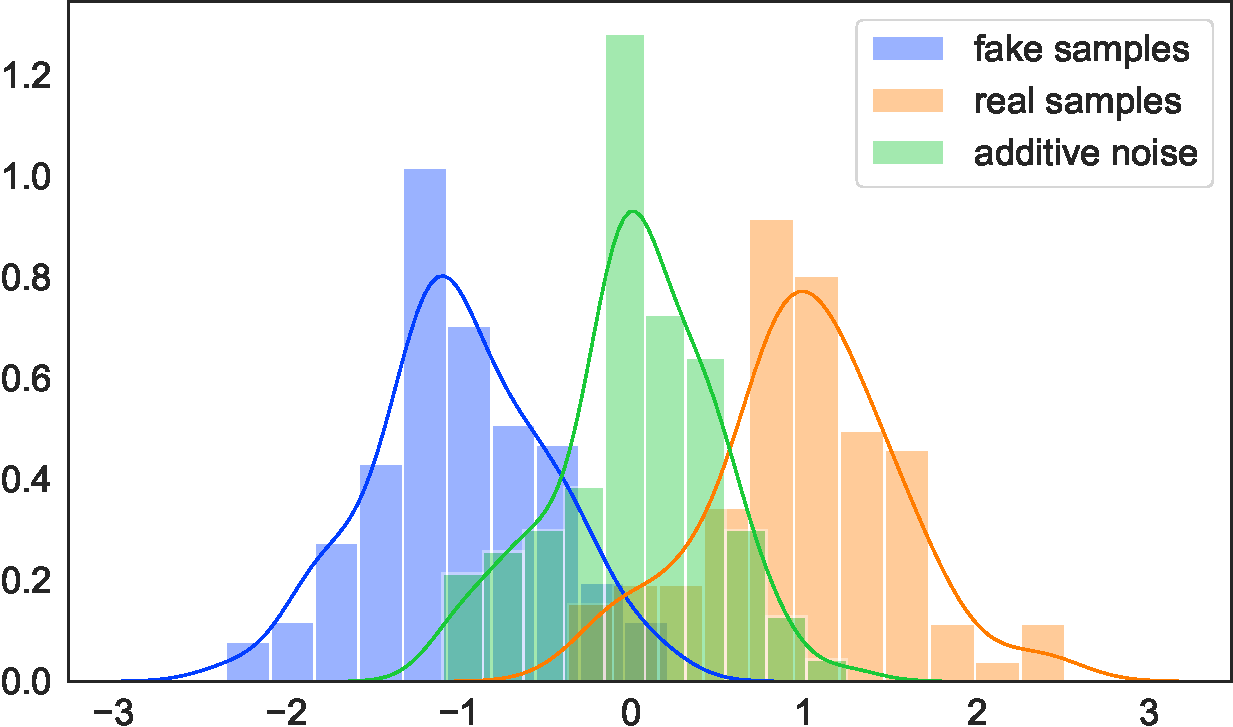
\includegraphics[width=0.48\textwidth,height=6cm]{additive-noise}%
	\caption{Visualizing the effect of Synthetic Noise Addition to the Discriminator Inputs}
	\label{fig:synthetic-noise}%
\end{figure}
\begin{figure*}[h!]
	\centering
	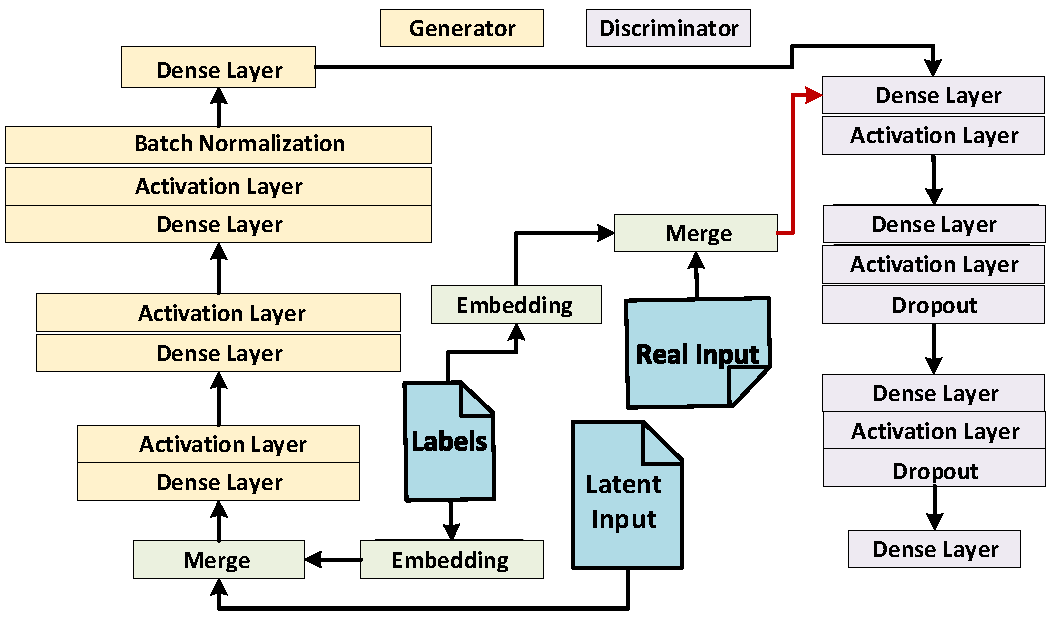
\includegraphics[width=0.96\textwidth,height=8cm]{GAN-Architecture}%
	\caption{Architecture of the Conditional Generative Adversarial Networks (CGAN) of AD-CGAN}%
	\label{fig:cgan}%
\end{figure*}
 Again, \cite{warrender1999detecting,hofmeyr1998intrusion} only consider the temporal 
\emph{ordering} of the traces and all other parameters like the timing 
information and system call arguments are ignored, and their approaches cannot 
handle a previously unseen system call without reconstructing the whole model.
\par
In \cite{li2019mad}, the authors implemented a generic GAN called MAD-GAN to do anomaly detection in multivariate data by using the linear combination of the residual errors of the generator and discriminator to create an anomaly threshold. This work is closely related to our work in principle but differs greatly in design and implementation. MAD-GAN uses the generic GAN architecture but we have a GAN architecture conditioned by an input sequence to create a classification model that evolves with the context of the application or process. MAD-GAN also differs from ours in terms of making anomaly decision. It uses both the \textit{generator} and \textit{discriminator} for both training and testing while we require only the \textit{generator} during the testing phase. Also, instead of using residual errors of the GANs for anomaly decision as done in \cite{li2019mad}, we came up with a cluster-based anomaly detector. Finally, in \cite{ezeme2019deepanom,ezeme2020framework}, the authors implemented an ensemble framework called based on the encoder-decoder model using attention layer to do anomaly detection in both the event and temporal stream of the system call properties. This work uses similar principle as our work but differs in architecture. Furthermore, \cite{ezeme2019deepanom,ezeme2020framework} algorithms' predictions could suffer from cumulative errors as a result of use of anomalous sub-sequence in the input samples.

\section{AD-CGAN: Design and Implementation}
\label{sec:design}
In this section, we discuss the design of AD-CGAN starting with the discussion of the qualities that a good anomaly detector should possess before we delve into the details of AD-CGAN design. We also include a list of symbols glossary for aid in deciphering the different concepts introduced in this section and beyond. \par   
Imbalanced data creates overfitting and introduces poor generalization on the test data. Therefore, efficiency of the performance of an algorithm has to take into account the distribution of the different classes being \textit{predicted} or \textit{classified} to ensure that the performance being claimed actually performs better than a random guess. For example, a dataset that has \textit{normal} class of $\bm{95\%} $ and \textit{anomalous} class of $ \bm{5\%} $ already has a $ \bm{95\%} $ accuracy using human guess. Also, since the aim of anomaly detection frameworks is to detect that critical $ \bm{5\%} $ of anomalous samples in this example, this $ \bm{95\%} $ performance accuracy in this regard may not make sense without taking into account the \textit{true negative, true positive} and other metrics that demonstrate how much of the critical samples were correctly detected. In some applications, the amount of human and capital resources required to investigate or deal with the effect of false positive classification is also huge, therefore, an effective anomaly framework should have the ability to detect the anomalous samples while reducing the incidents of false positives.
Having carefully considered the qualities that an anomaly detection framework should possess, we discuss the different modules of our \textit{AD-CGAN}. First, we discuss the inner-workings of the \textit{CGAN}s of Fig. \ref{fig:cgan} in Section \ref{subsec:gans} and in Section \ref{subsec:ad-cgan}, we discuss the complete architecture of the \textit{AD-CGAN} as shown in Fig. \ref{fig:ad-cgan}.
\glsaddall
\printglossary[title={List of Symbols}]  
\subsection{Conditional Generative Adversarial Networks}
\label{subsec:gans}
In this section, we discuss the modules of the CGAN with particular attention to the two main modules: \textit{generator}, and \textit{discriminator}.
\subsubsection{Generator}
\label{subsubsec:generator}
Our generator is a stack of artificial neural networks in which the number of cells doubled for each succeeding layer. The dense layer are sandwiched with activation layers and the last layer before the output layer has a \textit{batch normalization} layer as a \textit{regularization} scheme that makes the network robust and improve the \textit{generalization} properties of the network. Given a latent input, $ \bm{z} $, a conditional input, $ \bm{c} $, \eqref{eq:generator} is the generator equation where $ \bm{G} $ is a non-linear function like an artificial neural networks. The output, $ \bm{\vec{y}_{g}} $ of \eqref{eq:generator} is a sequence of multivariate data representing the context being modeled. 
\begin{equation}
	\bm{G:(\vec{z},\vec{c})}\longmapsto \bm{\vec{y}_{g}}
	\label{eq:generator}
\end{equation}
The $ \bm{\vec{y}_{g}} $ can be discrete, continuous or a mixture of both. As an additional stabilization measure to avoid mode collapse and overfitting, the output, $ \bm{\vec{y}_{g}} $ is augmented with a white noise as described in Section \ref{subsubsec:disc-overfit} before it is fed to the discriminator.
\subsubsection{Discriminator}
\label{subsubsec:discriminator}
In \cite{chen2016infogan}, it has been shown that some assumptions like finite log-likelihood-ratio between the generated data, $ \bm{\vec{y}_g} $ and the true value, $\bm{\vec{x}_d}  $, and the non-saturation of the Janson-Shannon divergence, $ \bm{JS[\vec{y}_g|\vec{x}_d]} $ to a maximum value do not hold in most cases. Therefore, an additive noise from a normal distribution with varying variance ensures that the discriminator does not overfit during training. We added the noise to each sample, $ \bm{y_g \in \vec{y}_g} $ and $ \bm{x_d \in \vec{x}_d} $ because adding it to the generated output only could also aid the discriminator in overfitting on the training data. In the discriminator model of Fig. \ref{fig:cgan}, we use \textit{dropout} in the second and third layers to reduce overfitting by reducing the \textit{interdependent learning} amongst the neurons. In \eqref{eq:discriminator}, we provide the equation which captures the relationship between the input and output of the discriminator.
\begin{equation}
\bm{D:(\vec{y}, \widetilde{x})}\longmapsto \bm{\vec{y}_{d}} \:
\text{where}\; \bm{\vec{y}} \supseteq \bm{\vec{y}_g,\vec{x}_d}
\label{eq:discriminator}
\end{equation} 
 
During training, AD-CGAN objective loss function that captures the relationship between the generator and discriminator is given in \eqref{eq:obj-func} where $ \bm{L_G} $ and $ \bm{L_D} $ represent the generator and discriminator loss respectively.
\begin{equation}
\label{eq:obj-func}
\begin{aligned}
\bm{L_D} &= \bm{E[\log(D(\vec{x}_d,\widetilde{x}))]}\\
	& \bm{+E[\log(1-D(G(\vec{z},\vec{c}),\widetilde{x}))]} \\\\
\bm{L_G} &= \bm{E[\log(D(G(\vec{z},\vec{c}),\widetilde{x})))]}
\end{aligned}
\end{equation}
\begin{figure*}[h!]
	\centering
	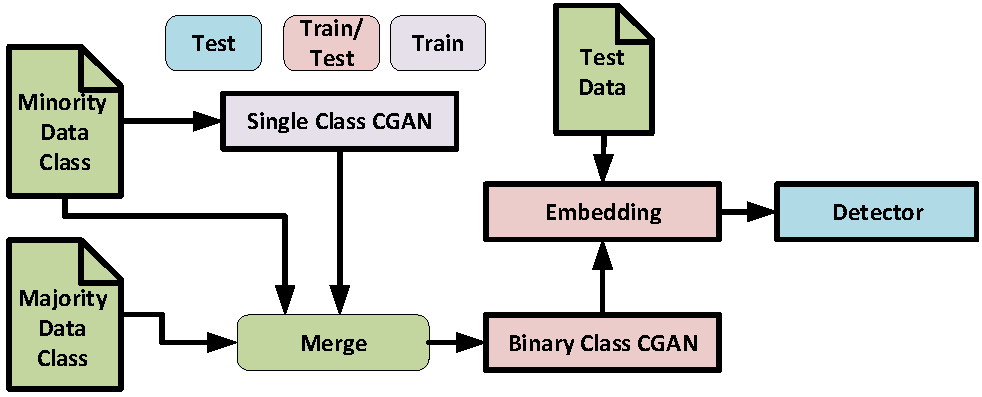
\includegraphics[width=0.96\textwidth,height=8cm]{AD-CGAN}%
	\caption{AD-CGAN Framework for Anomaly Detection in Balanced and Imbalanced Data}
	\label{fig:ad-cgan}%
\end{figure*}
\subsubsection{Controlling Discriminator Overfitting}
\label{subsubsec:disc-overfit}
In Fig. \ref{fig:synthetic-noise}, we show the effect of adding synthetic noise to both the generator output, $ \bm{\vec{y}_g} $ and the real samples input, $ \bm{\vec{x}_d} $. One of the underlying assumptions of GANs is that the log-likelihood ratio $ \log \dfrac{\vec{y}_g(\vec{y_d})}{\vec{x}_d(\vec{y}_d)} $ is finite. However, in some chaotic real world scenarios, given $\bm{G:(\vec{z},\vec{c})}\longmapsto \bm{\vec{y}_{g}}  $ where the support is $ \{\bm{z\in\vec{z},c\in\vec{c}:G(z,c)\neq0}\} $, the intersection between the support of the generator and the support of the distribution that produced $ \bm{\vec{x}_d} $ in high dimensional space may be $ \emptyset $ if the underlying distributions are \textit{degenerate}. Hence, the addition of synthetic noise as shown in \eqref{eq:discriminator} aims to create an overlapping support for the two underlying distributions. This ensures that the log-likelihood remains finite and Jensen-Shannon divergence produces a continuous function which does not saturate to a constant value. Thereby reducing overfitting in the discriminator.

\subsection{AD-CGAN}
\label{subsec:ad-cgan}
The main blocks of Fig. \ref{fig:ad-cgan} are \textit{single class CGAN, binary class CGAN, Embedding,} and the \textit{Detector}. In the following sections, we highlight the role of each modules in the overall functionality of the \textit{AD-CGAN}. 
\subsubsection{Single Class CGAN}
\label{subsub:scgan}
Given a dataset for training that consists of \textit{normal} and \textit{anomalous} profiles, we determine the number of samples of each category. If the ratio of the majority class to the minority class is high and could introduce bias in the model, we learn the profile of the minority class using the \textit{single class CGAN}. With the the single class CGAN trained on the minority class, we use it to generate more data samples of the minority class to augment the number of the minority class samples until the data samples of the majority and minority class samples are fairly even. The aim of the single class CGAN is to train the generator, $ \bm{G_s} $ with the multivariate data, $ \bm{\vec{z}, \vec{c}} $ so that the generator output, $ \bm{\vec{y}_g} $ and the real samples of the class of interest, $\bm{\vec{x}_d}$ when clustered, show evidence that $\bm{\vec{x}_d}$ and $ \bm{\vec{y}_g} $ are drawn from the same underlying distribution. We measure this similarity with the use of the \textit{stochastic neighbor embedding} algorithm \cite{hinton2003stochastic}. As will be shown in Section \ref{sec:experiments}, when the single class CGAN is sufficiently trained, the generator output, $ \bm{\vec{y}_g} $ and the real samples, $ \bm{\vec{x}_d} $ form a single indistinguishable cluster.
\subsubsection{Binary Class CGAN}
\label{subsub:bcgan}
The \textit{binary class CGAN} trains on the \textit{normal} and \textit{anomalous} samples from the original and augmented samples from the \textit{single class CGAN}. Unlike the the single class CGAN, the aim of the binary class CGAN is to train the generator, $ \bm{G_b} $ with the multivariate binary class data, $ \bm{\vec{z},\vec{c}} $ such that the anomalous samples from the generator output, $ \bm{\vec{y}_g} $, and the anomalous samples of the real samples, $ \bm{\vec{x}_d}$ form a single distinct cluster while the corresponding normal samples from both the generator and the real samples form a different, distinct cluster. Therefore, we can say that the major difference between the \textit{single class CGAN} and the \textit{binary class CGAN} is that the former trains to \textit{merge} two samples that belong to the same class while the latter trains to \textit{fuse} the same class samples in one cluster and \textit{diverge} different class samples to a different cluster. Therefore, the output of the single class CGAN is a single cluster while the binary class CGAN produces two clusters.
\subsubsection{Embedding} 
\label{subsub:tsne}
When we need to test some given samples, the binary class CGAN generates a matching number of samples comprising of both \textit{fake normal} and \textit{fake malicious} profiles, and this output, $ \bm{\vec{y}_g} $ is a multivariate data of the same dimension as the real samples, $ \bm{\vec{x}_d} $. Therefore, the number of samples generated by the binary class CGAN, $ \bm{\vec{y}_g} $ is the same as the number of the real samples, $ \bm{\vec{x}_d} $. The significance of using the binary class CGAN output in the embedding are: 
\begin{enumerate*}[label={\alph*)},font={\bfseries}]
	\item when plotted using a visualization tool during training, it gives us an idea of how the CGANs are able to learn the profiles of the data being studied;
	\item during testing, the \textit{fake labels} used in the CGANs to generate $ \bm{\vec{y}_g} $ guide us in constructing the different centroids of each class by giving us the ability to separate the \textit{fake normal} samples from the \textit{fake malicious} samples in the generated data.
\end{enumerate*} 
But while the dimension of the real sample, $ \bm{\vec{x}_d} $ is fixed, AD-CGAN can handle data of arbitrary dimension by \textit{preprocessing} the arbitrary dimensional data to the dimension of the real samples, $ \bm{\vec{x}_d} $ using the sparse principal component analysis algorithm \cite{zou2006sparse}. Furthermore, we use the stochastic neighbor embedding algorithm to ensure that points in the high-dimensional space correspond to nearby embedded low-dimensional points, and distant points in high-dimensional space correspond to distant embedded low-dimensional points. Given $ \bm{ \{\vec{y}_g, \vec{x}_d\} \in \vec{y}  } $, \eqref{eq:tsne} shows the neighbor embedding algorithm which we employ to compute the conditional probabilities, $ \bm{P_{j|i}} $ that highlights the probability of  point $ \bm{j} $ choosing point $ \bm{i} $ as a neighbor.
\begin{equation}
	\bm{P_{j|i}} = \bm{\frac{exp\left(- \nicefrac{\abs{y_i - y_j} ^2}{2\sigma_i^2}    \right)}{ \sum_{k\neq i} exp\left(- \nicefrac{\abs{y_i - y_k} ^2}{2\sigma_i^2}    \right)}}
	\label{eq:tsne} 
\end{equation}
To ensure symmetry, we compute the \textit{joint} probability, $ \bm{P_{ij} }$ of the similarity between points $ \bm{i} $ and $ \bm{j} $ using \eqref{eq:jptsne}. Since $ {\bm{P_{j|j}=0} }$, $ \bm{P_{jj}=0} $ in \eqref{eq:jptsne}. In this work, our neighbor embedding algorithm of \eqref{eq:tsne} produces embedding output in two dimensions so as to make it easy to use visualization tools to inspect the performance of the CGAN networks. 
\begin{equation}
	\label{eq:jptsne}
	\bm{P_{ij}}=\bm{\frac{P_{j|i}+P_{i|j}}{2N}} \;
	\text{where}\; N=\text{number of rows of}\; \bm{\vec{y}}
\end{equation}
\begin{figure*}
	\centering
	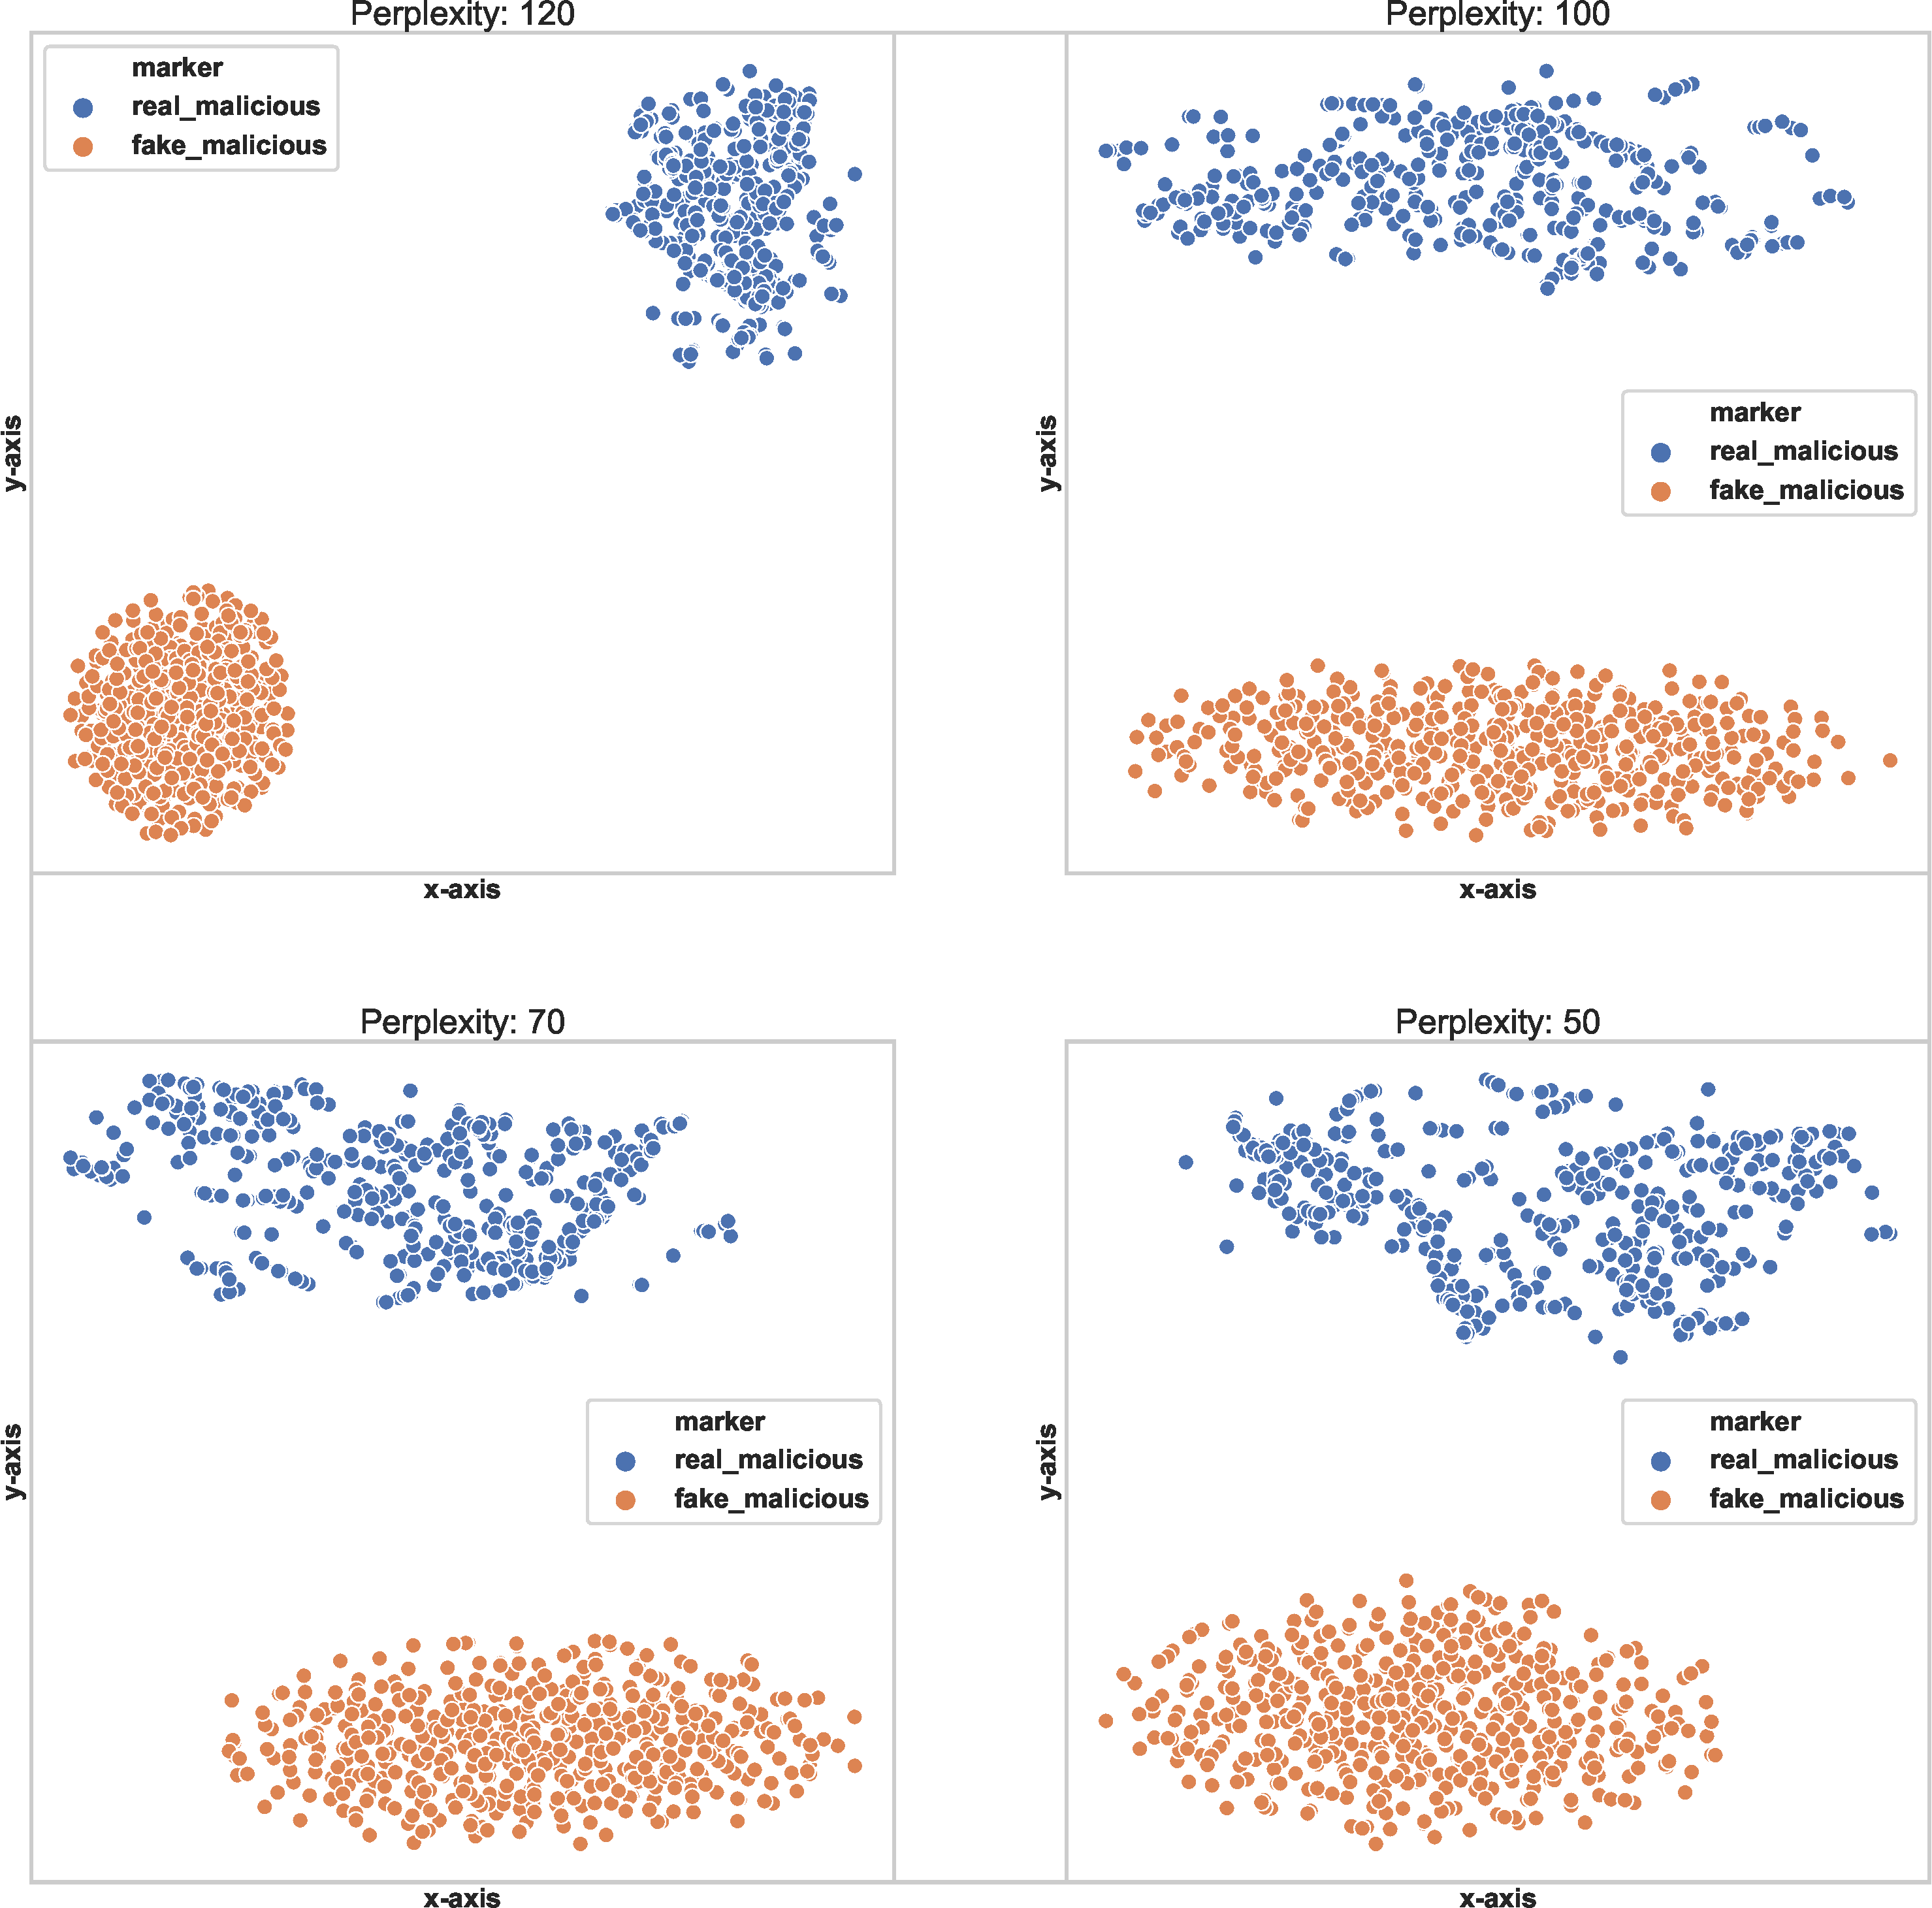
\includegraphics[width=\textwidth,keepaspectratio]{aloi-a-untrained}
	\caption{Before Training (ALOI): Real and Fake Samples of the Single Class CGAN form $ \bm{2} $ Clusters}
	\label{fig:aloi-a-untrained}
\end{figure*}
\begin{figure*}
	\centering
	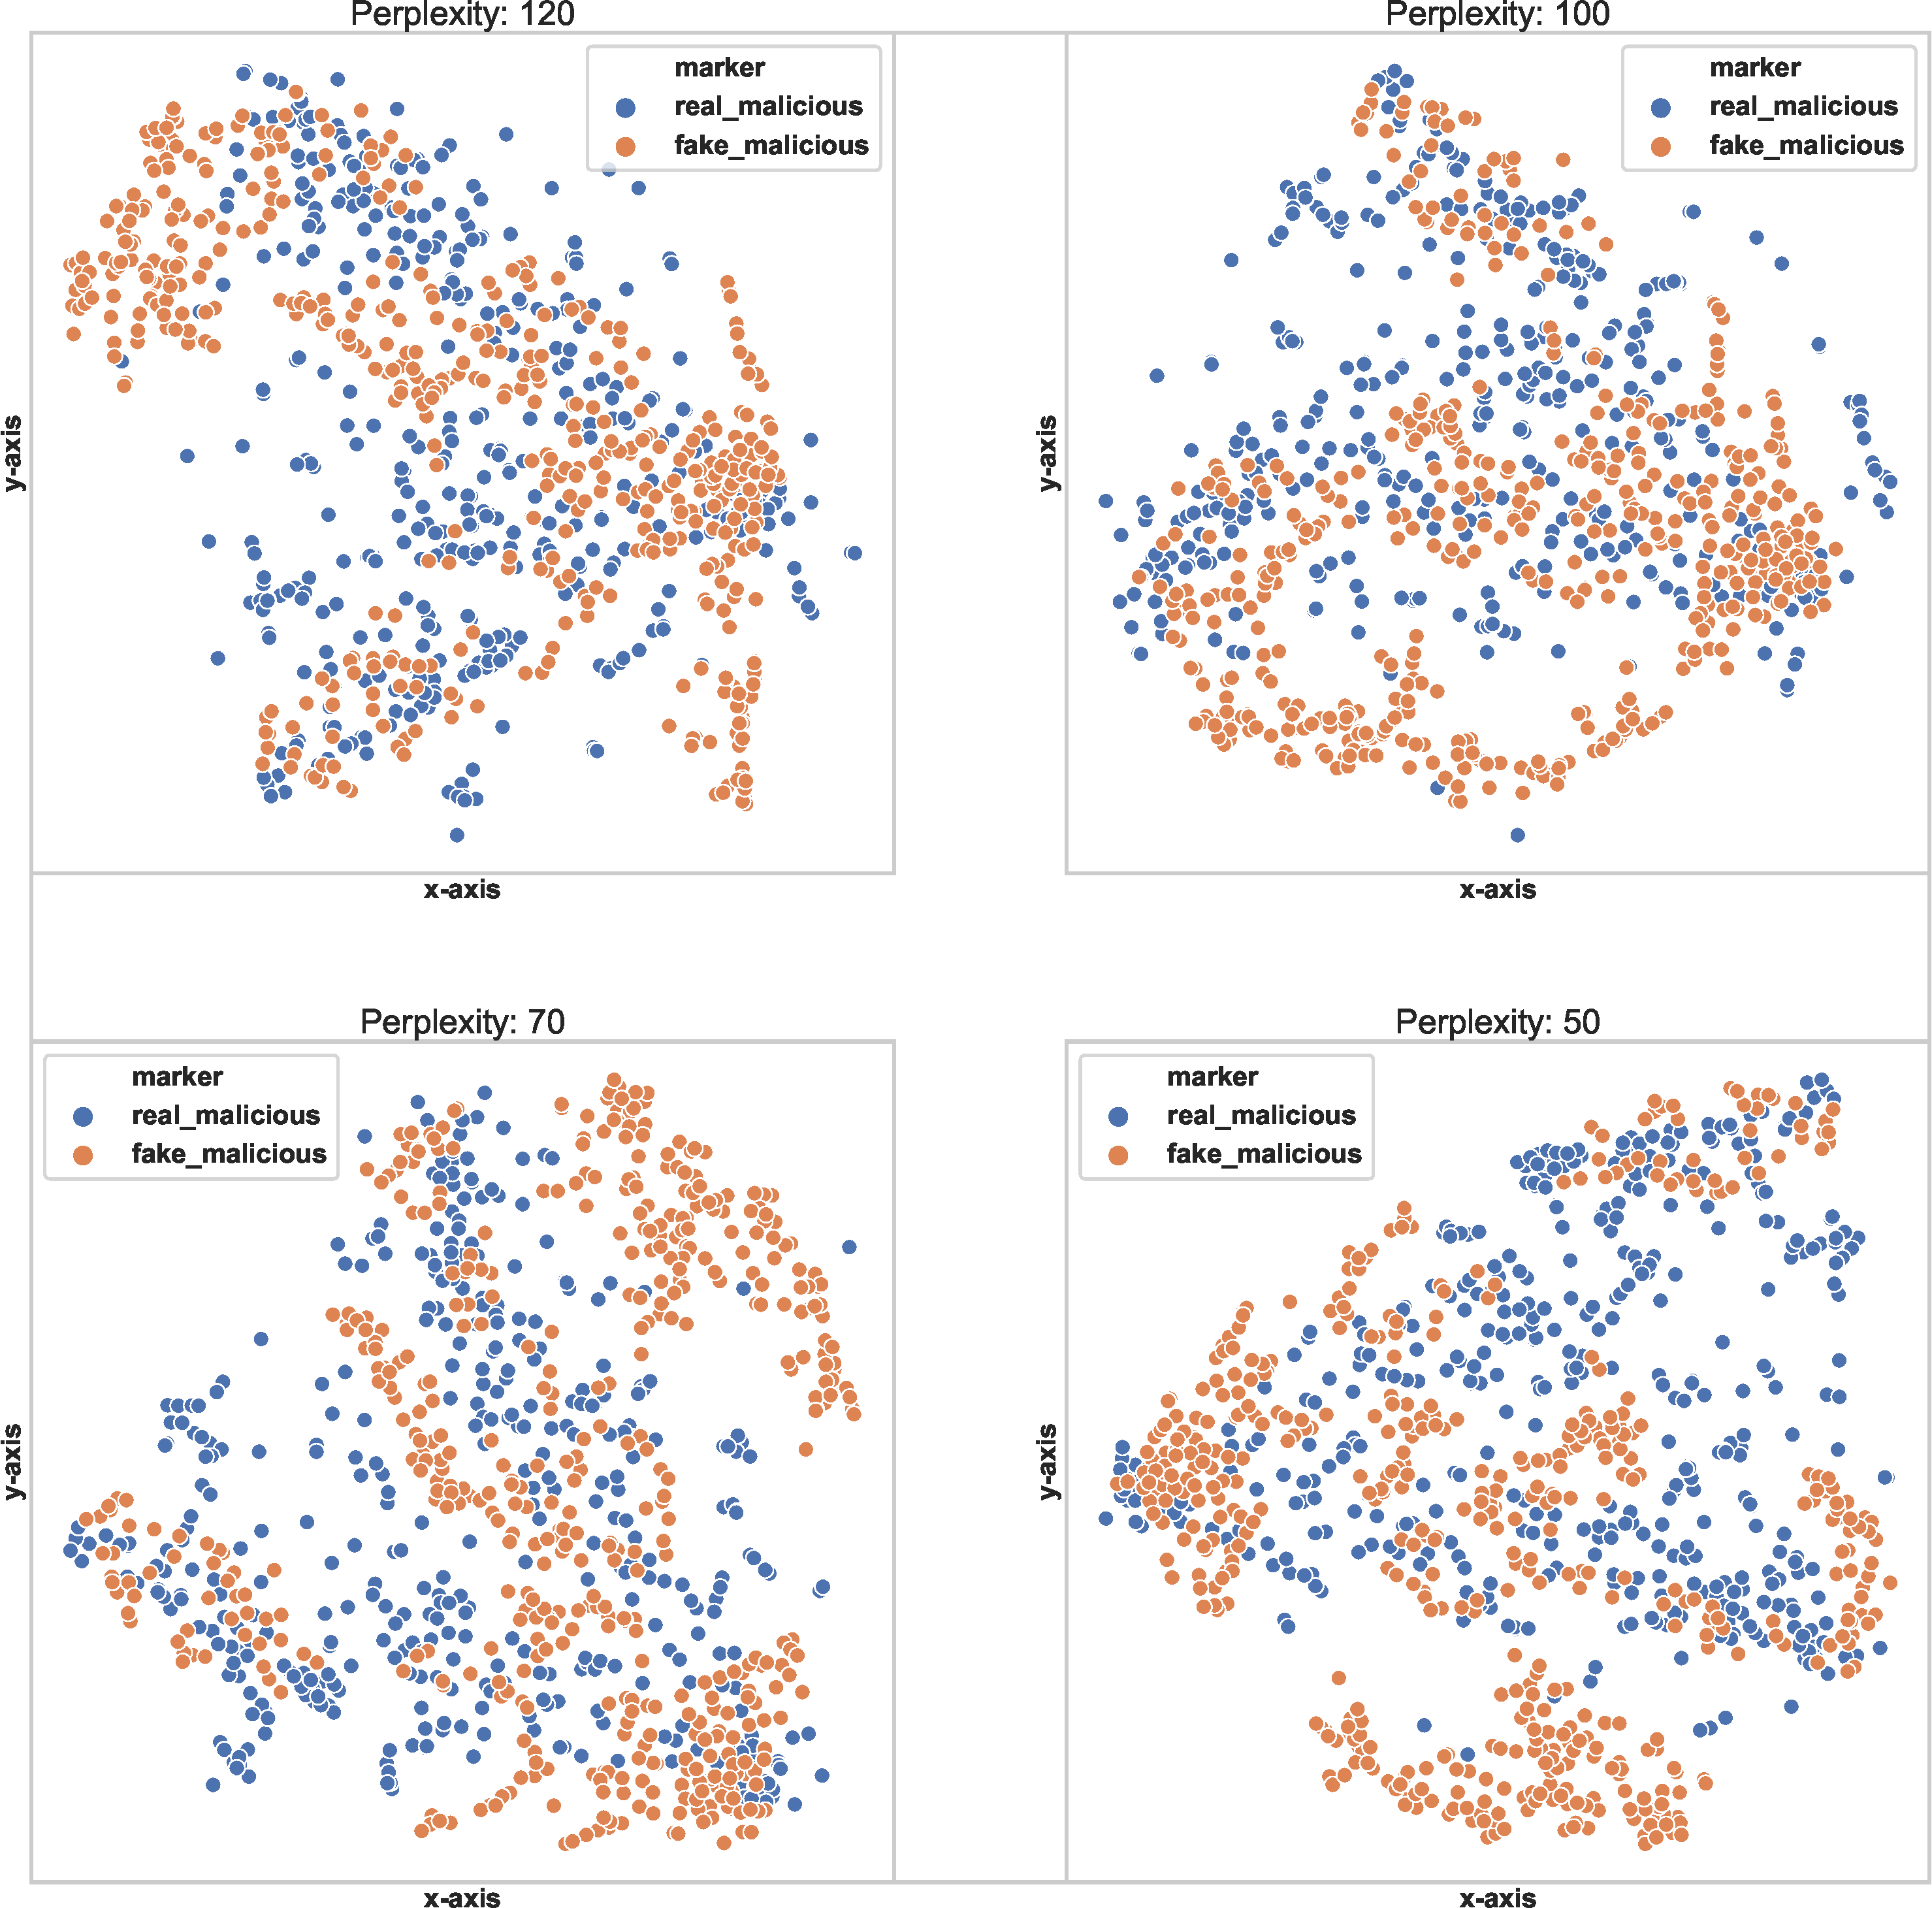
\includegraphics[width=\textwidth,keepaspectratio]{aloi-a-trained}
	\caption{After Training (ALOI): Real and Fake Samples of the Single Class CGAN form $ \bm{1} $ Cluster}
	\label{fig:aloi-a-trained}
\end{figure*}
\begin{figure*}
	\centering
	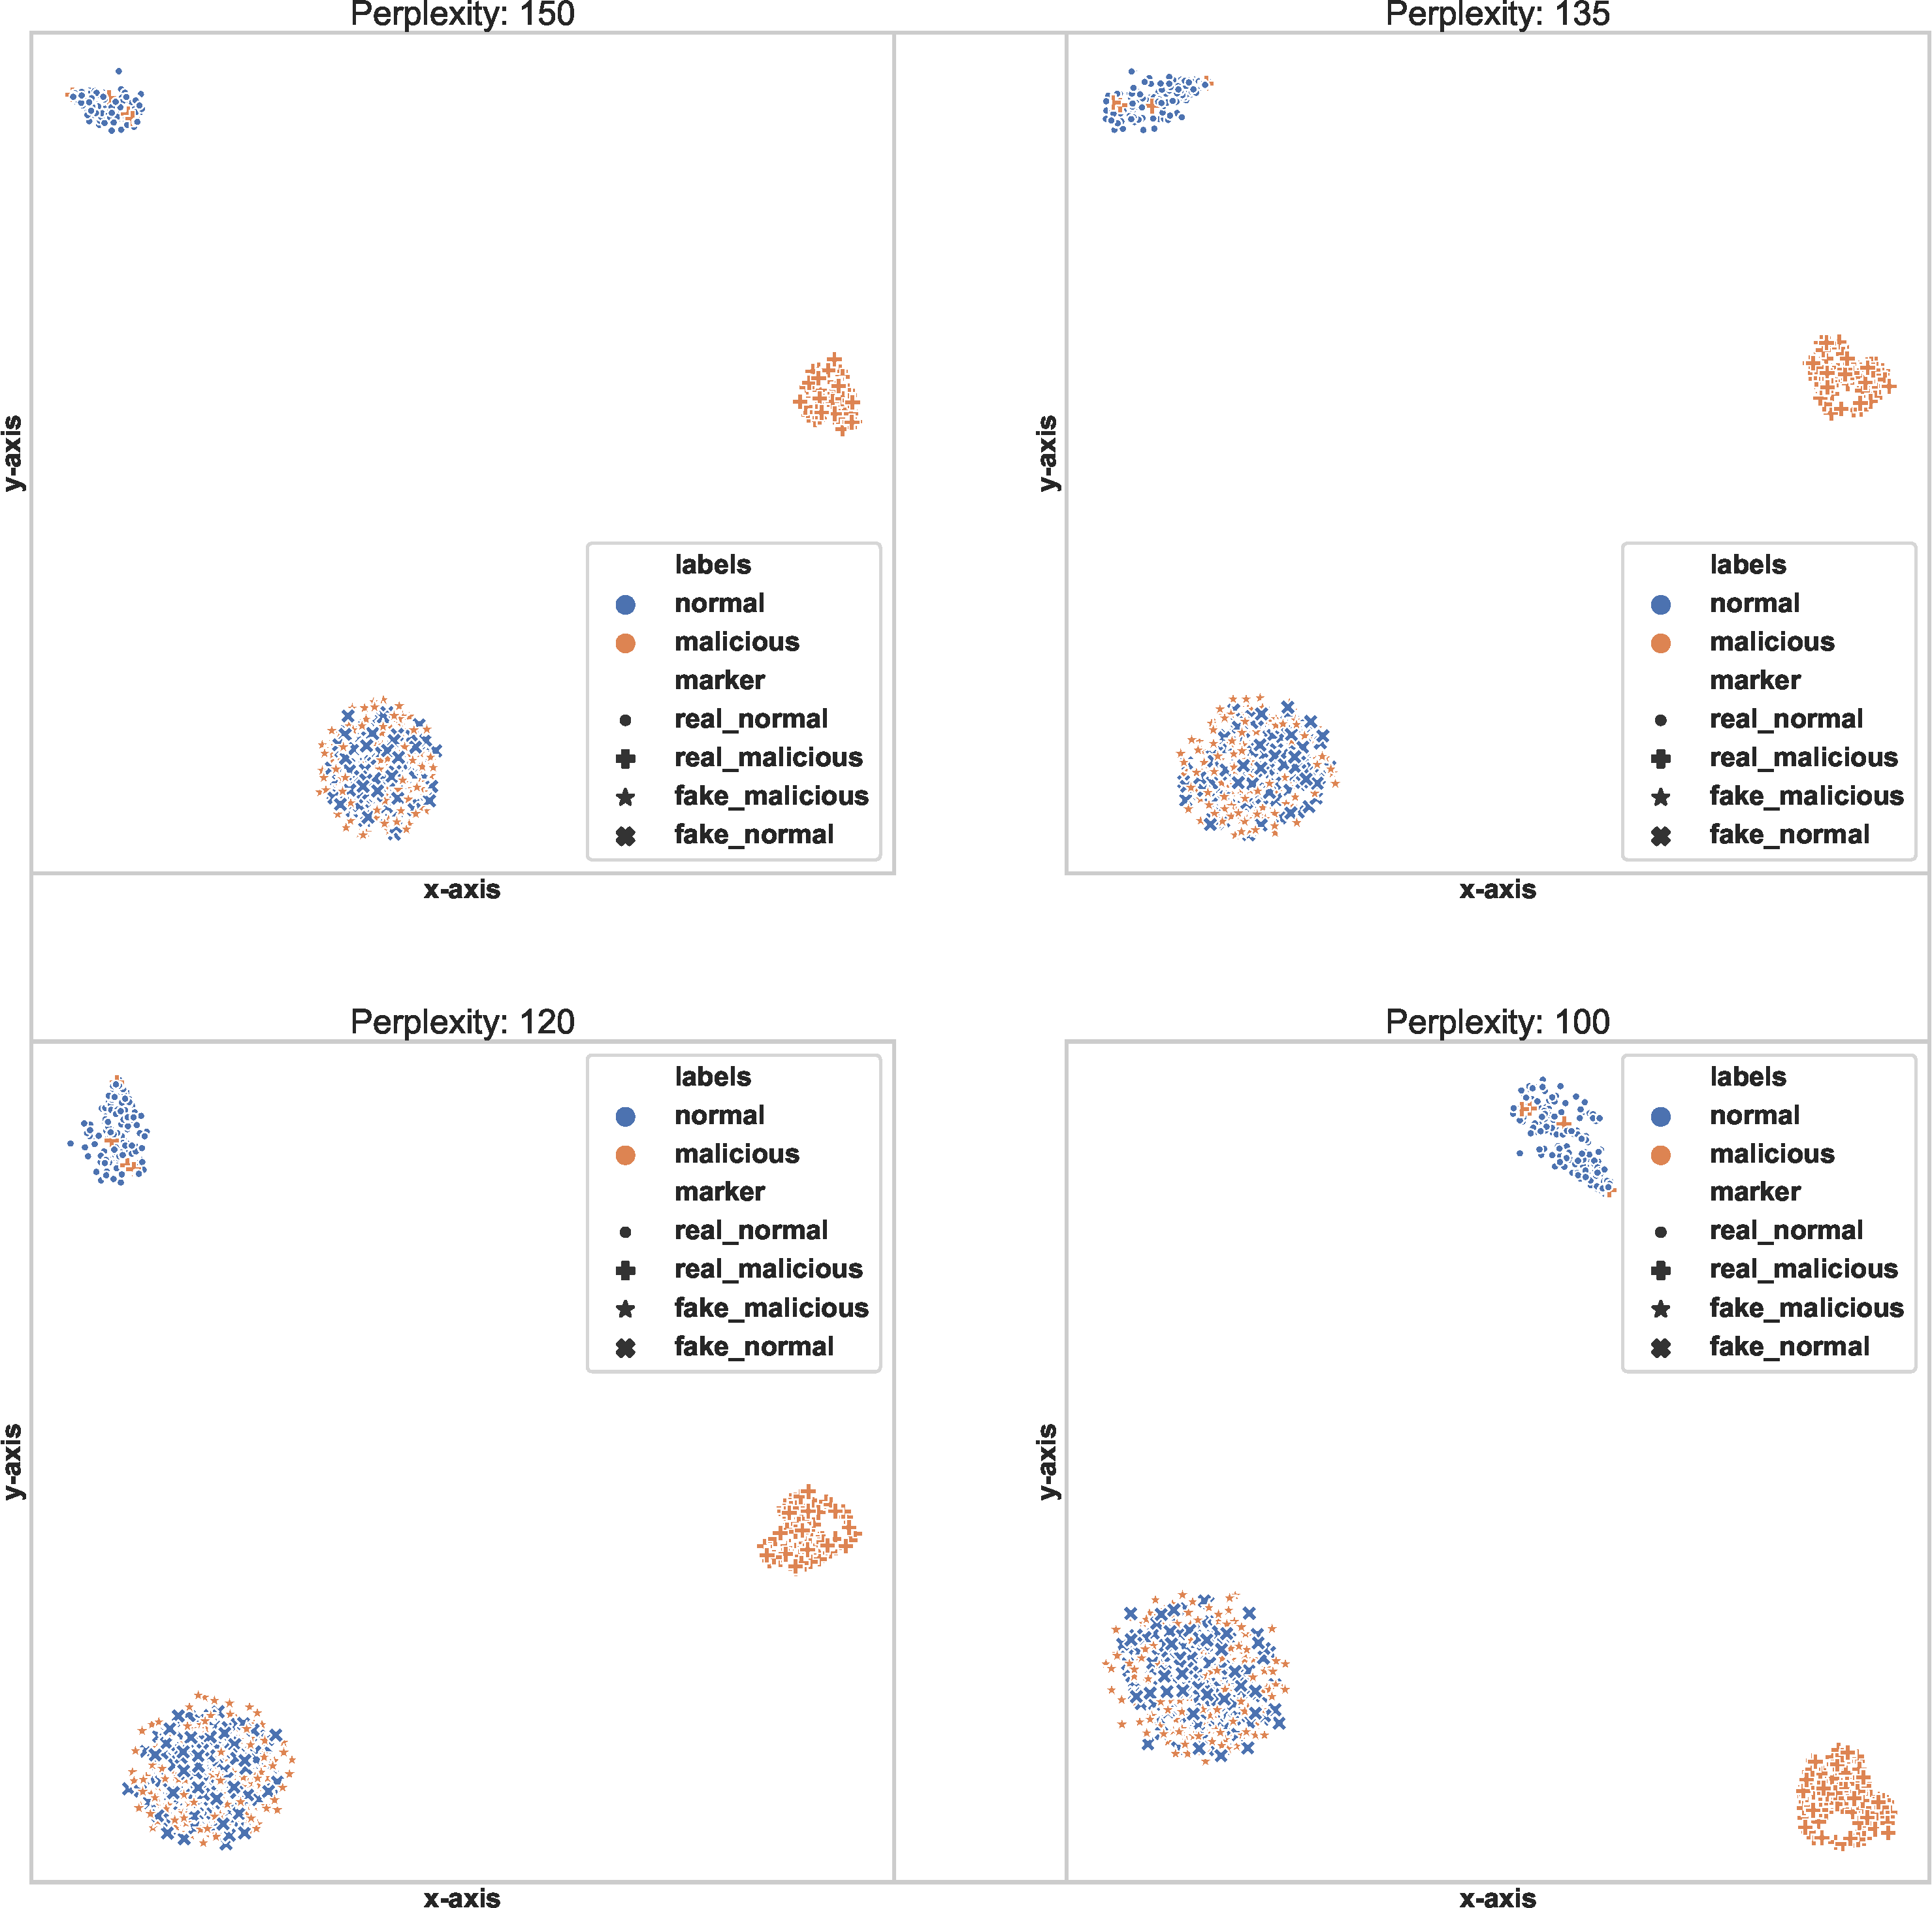
\includegraphics[width=\textwidth,keepaspectratio]{aloi-untrained}
	\caption{Before Training (ALOI): Binary Class CGAN generates Mixed Clusters for Malicious and Normal Profiles}
	\label{fig:aloi-untrained}	
\end{figure*}
\begin{figure*}
	\centering
	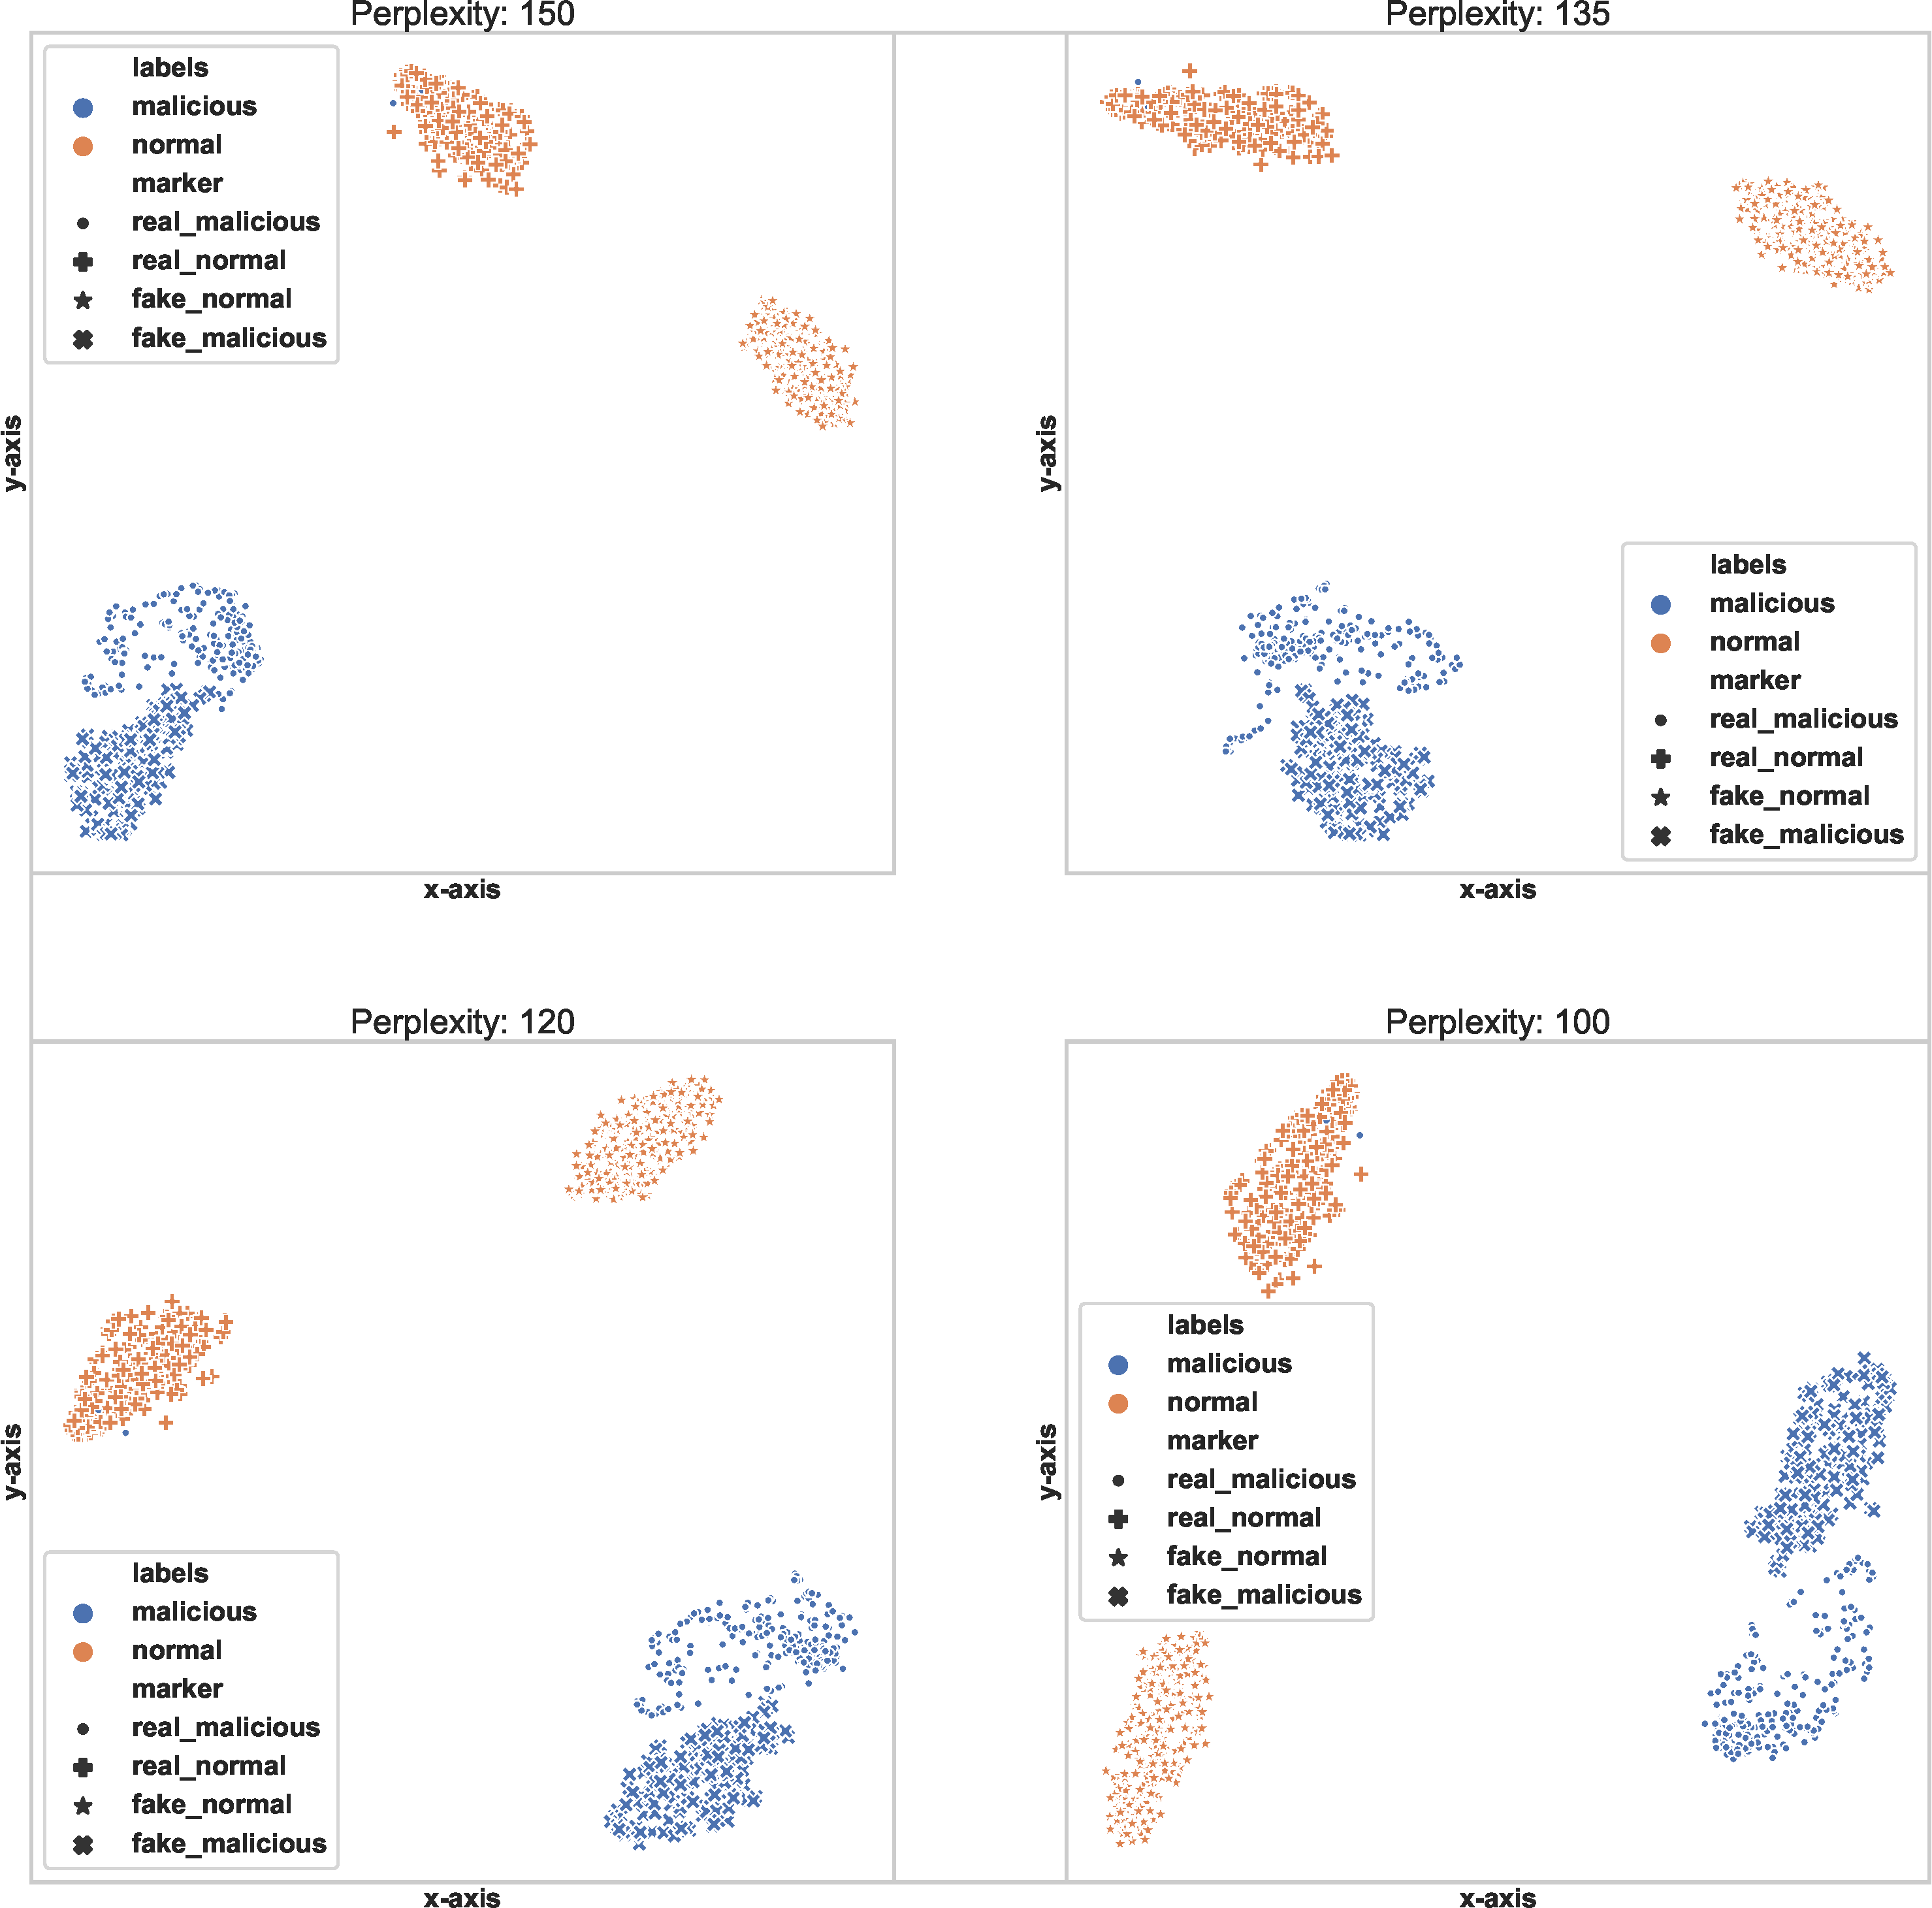
\includegraphics[width=\textwidth,keepaspectratio]{aloi-trained}
	\caption{After Training (ALOI): Binary Class CGAN generates Distinct Clusters for the Malicious and Normal Profiles }
	\label{fig:aloi-trained}
\end{figure*}
\subsubsection{Detector}
\label{subsub:detector} 
From Fig. \ref{fig:ad-cgan}, \eqref{eq:tsne-transform} represents the embedding from higher to lower two-dimensional space. The resulting output is a set, $ { \bm{S=\{(m_1,n_1),(m_2,n_2),...,(m_t,n_t)\}}} $ of tuples of point coordinates of both the real and generated samples. 
\begin{equation}
\label{eq:tsne-transform}
\bm{f:\mathbb{R}^{p\times q}\longmapsto\mathbb{R}^{p\times 2}}\; \text{where}\; \bm{p=} \text{number of samples}
\end{equation}
During evaluation, we use the labels used in the CGAN generator to separate the coordinates of the fake normal samples from the fake anomalous samples, and compute the centroid of each class using \eqref{eq:centroid} on the fake samples only. 
\begin{equation}
	\label{eq:centroid}
	\bm{\left(\bar{m}_i,\bar{n}_i\right)}=\bm{\left( \frac{1}{t}\sum_{j=0}^{t}m_{ji},\frac{1}{t}\sum_{j=0}^{t}n_{ji}\right)} \; \forall\; i\in \{0,1\}
\end{equation}
Using \textit{t-statistics}, we derive the distance of new points being tested from the centroid using \eqref{eq:subtraction} where $ \bm{\sigma_{s}} $ and $ \bm{\left(\bar{m}_s,\bar{n}_s\right)} $ are the evaluation sample standard deviation and mean respectively. Since the centroid is a vector, computing distance becomes simple vector subtraction standardized using the standard deviation as shown in \eqref{eq:subtraction}. For simplification purposes, we use the norm of the output of \eqref{eq:subtraction} to measure the absolute distance from each of the two classes.
\begin{equation}
	\label{eq:subtraction}
	\bm{\left( \hat{m}_i,\hat{n}_i \right)}= \bm{\left( \frac{m_i-\bar{m}_i}{\sigma_{s_{mi}}}, \frac{n_i-\bar{n}_i}{\sigma_{s_{ni}}} \right)} \; \forall\; i\in \{0,1\}
\end{equation}
Therefore, anomaly detection decision is taken using \eqref{eq:decision} which selects the cluster with the highest probability score from the test point as the test point cluster. In \eqref{eq:decision}, $ \bm{C_k} $ is defined in \eqref{eq:bernoulli}. 
\begin{equation}
\bm{p_{2_i}}=\bm{\sqrt{\hat{m}_{i}^2+\hat{n}_{i}^2}} \; \forall\; i\in \{0,1\}
\label{eq:norm}
\end{equation}
In cases where the distance is equal from the two clusters, we break the tie by using \eqref{eq:bernoulli} to select a cluster for the test point. In \eqref{eq:scores}, we compute the probability of the test point belonging to any of the clusters using the distances of \eqref{eq:norm}. 
\begin{equation}
\label{eq:scores}
\bm{P(i) = \frac{p_{2_i}}{\sum_{i}^{n}p_{2_i}}}\; \forall\; i\in \{0,1\}
\end{equation}
Then, we determine which cluster the test point belongs to using the probabilities of \eqref{eq:scores} and \eqref{eq:bernoulli} in \eqref{eq:decision}.

\begin{equation}
\label{eq:bernoulli}
\bm{C_k} = \left\{
\begin{array}{lr}
\bm{C_0 = 1-C_1}, & \text{if } \bm{k=0} \\
\bm{C_1}, & \text{if }  \bm{k=1}
\end{array}
\right.
\end{equation}
Since the \textit{single class CGAN} has been used to do data augmentation, the evaluation data samples used to generate the centroids are balanced, hence, the justification for the use of the Bernoulli probability distribution selection when a tie occurs. As the context changes, we update the centroids via \textit{batch training} with the new data collected from the network. 
\begin{equation}
\label{eq:decision}
\bm{C_i} = \left\{ 
\begin{array}{lr}	
\bm{C_0}, & \bm{P(1) < P(0)} \\
\bm{C_1}, & \bm{P(0) < P(1)} \\
\bm{C_k}, & \bm{P(1) == P(0)}
\end{array}
\right.  
\end{equation}
This parameter update can be done in parallel with the deployed algorithm. When a new set of model parameters are generated, we update the model by copying the new parameters to our deployed framework.
\begin{figure*}
	\centering
	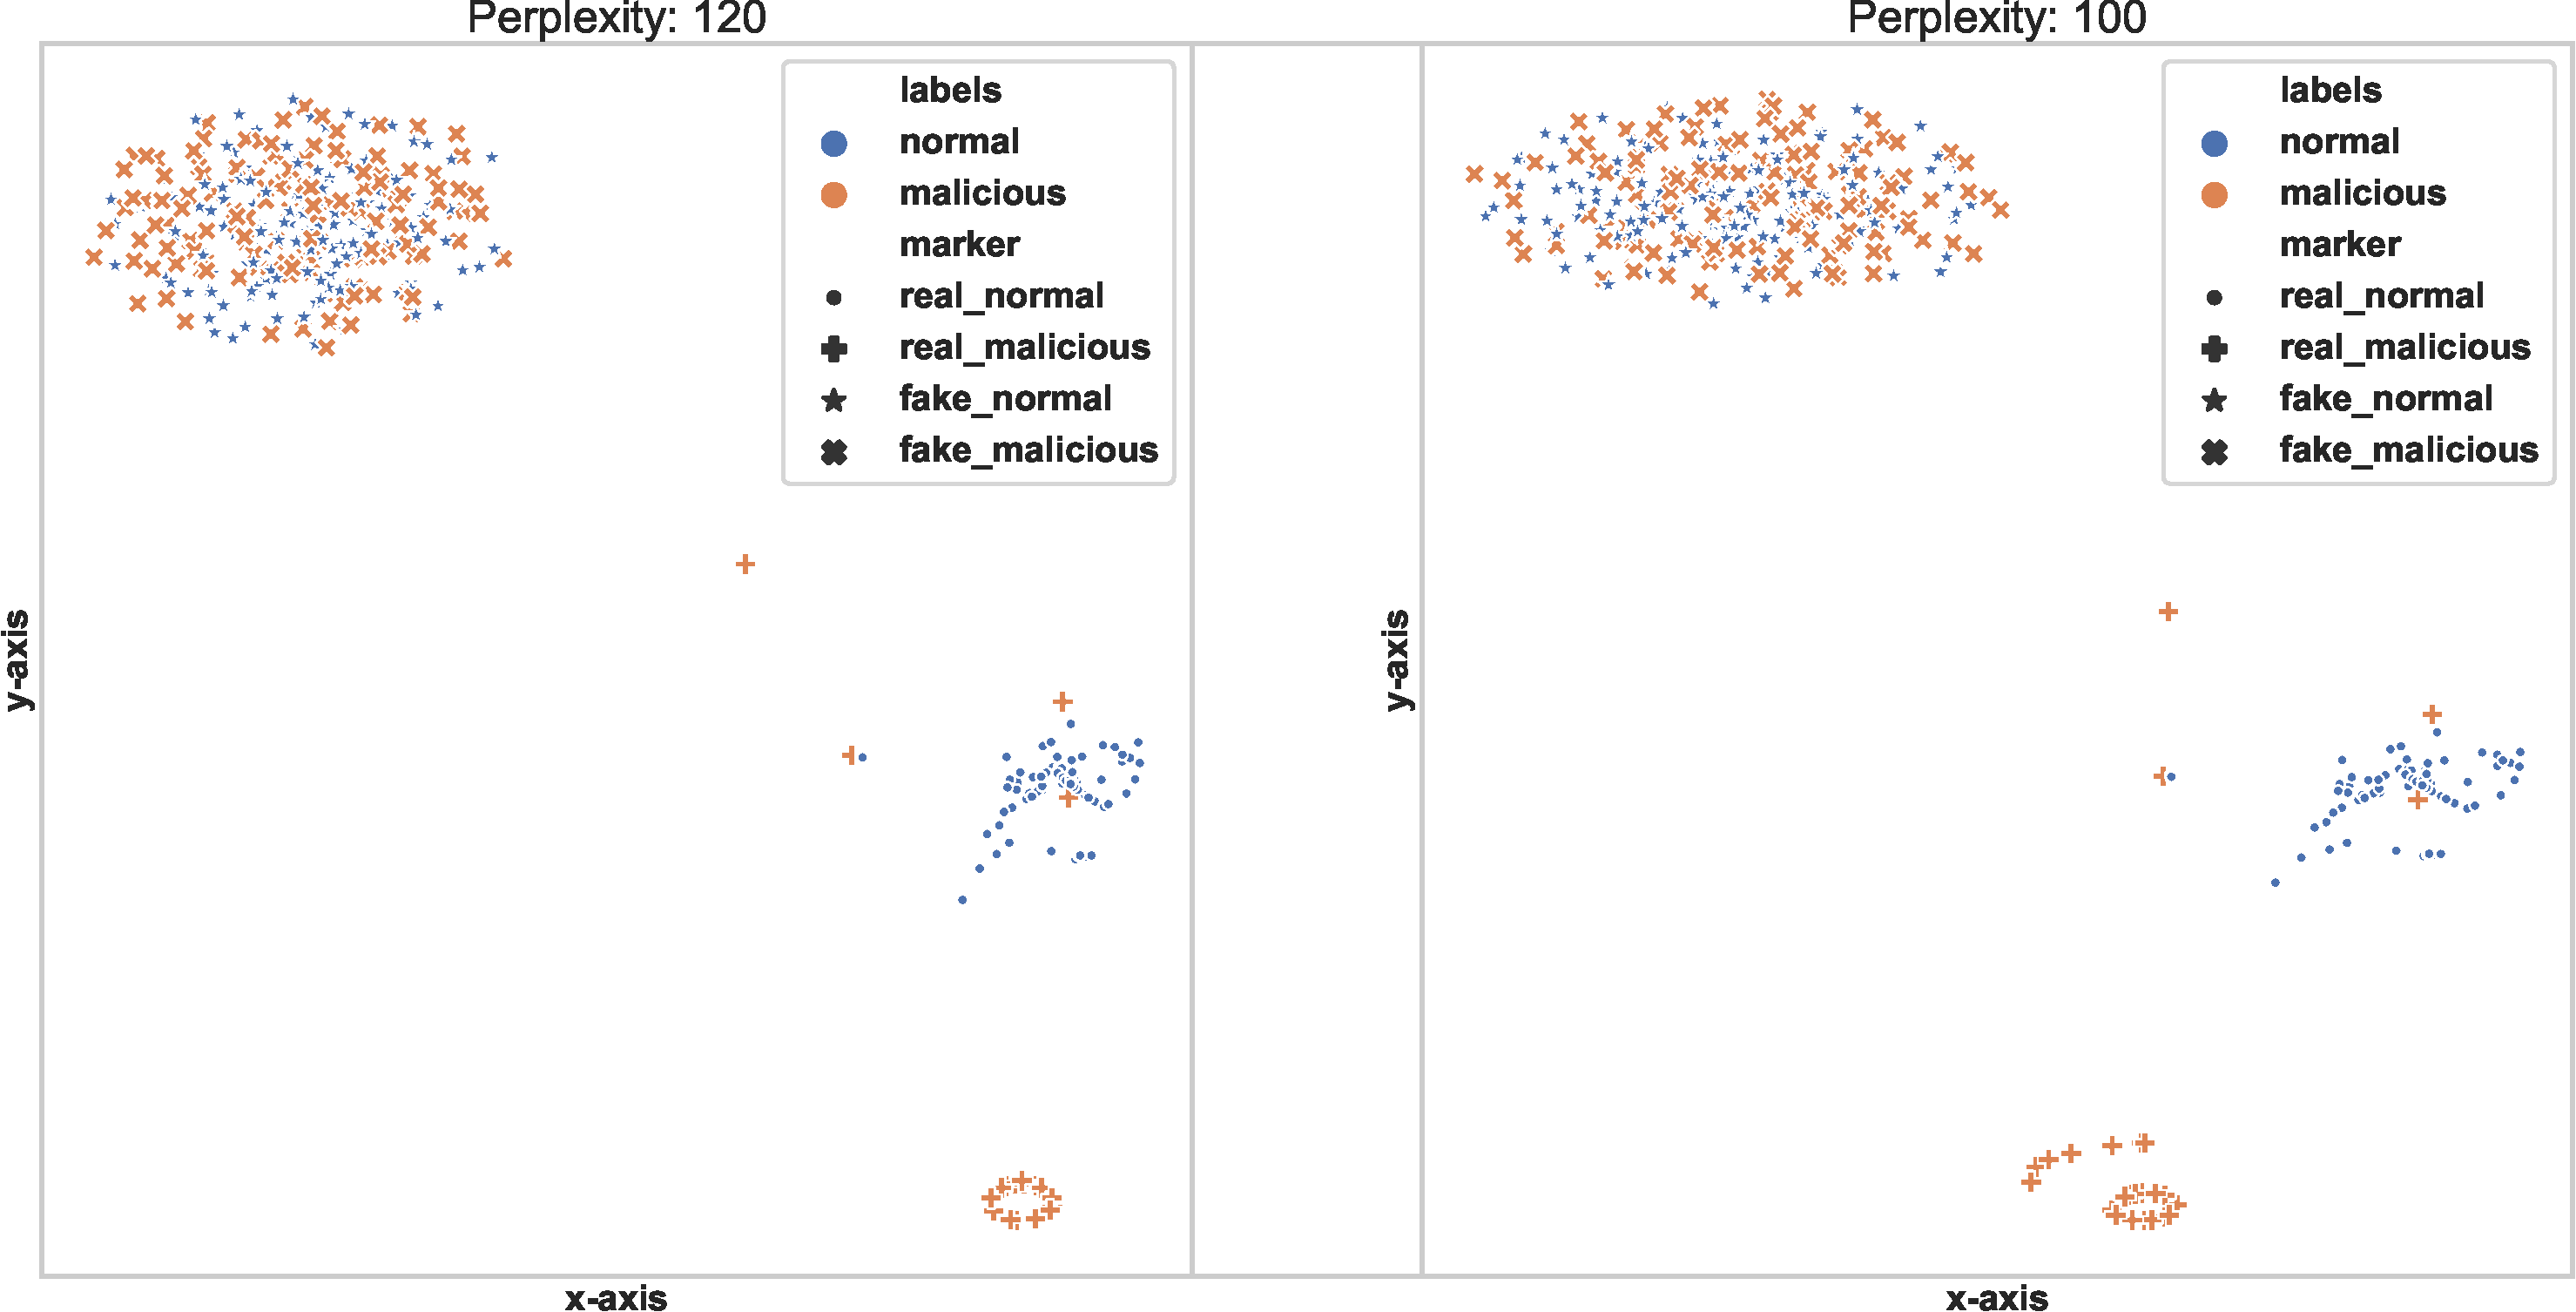
\includegraphics[width=\textwidth,keepaspectratio]{kdd-untrained}
	\caption{Before Training (KDD99): Binary Class CGAN creates Mixed Clusters for the Malicious and Normal Profiles}
	\label{fig:kdd-untrained}
\end{figure*}
 \begin{figure}[h!]
	\centering
	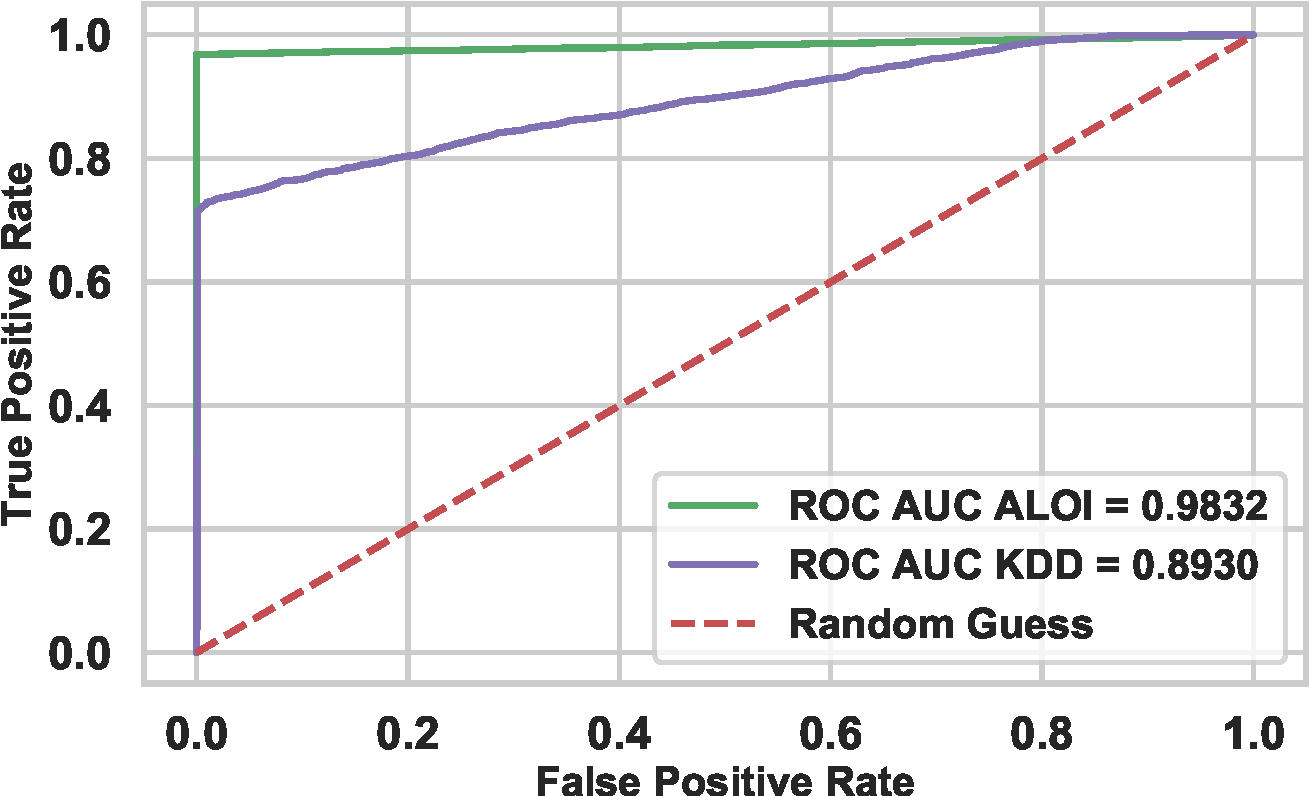
\includegraphics[width=0.50\textwidth,height=6cm]{auc_curve}%
	\caption{ROC Curve for the ALOI and KDD99 Dataset}
	\label{fig:auc-curve-aloi}%
\end{figure}
\begin{figure*}
	\centering
	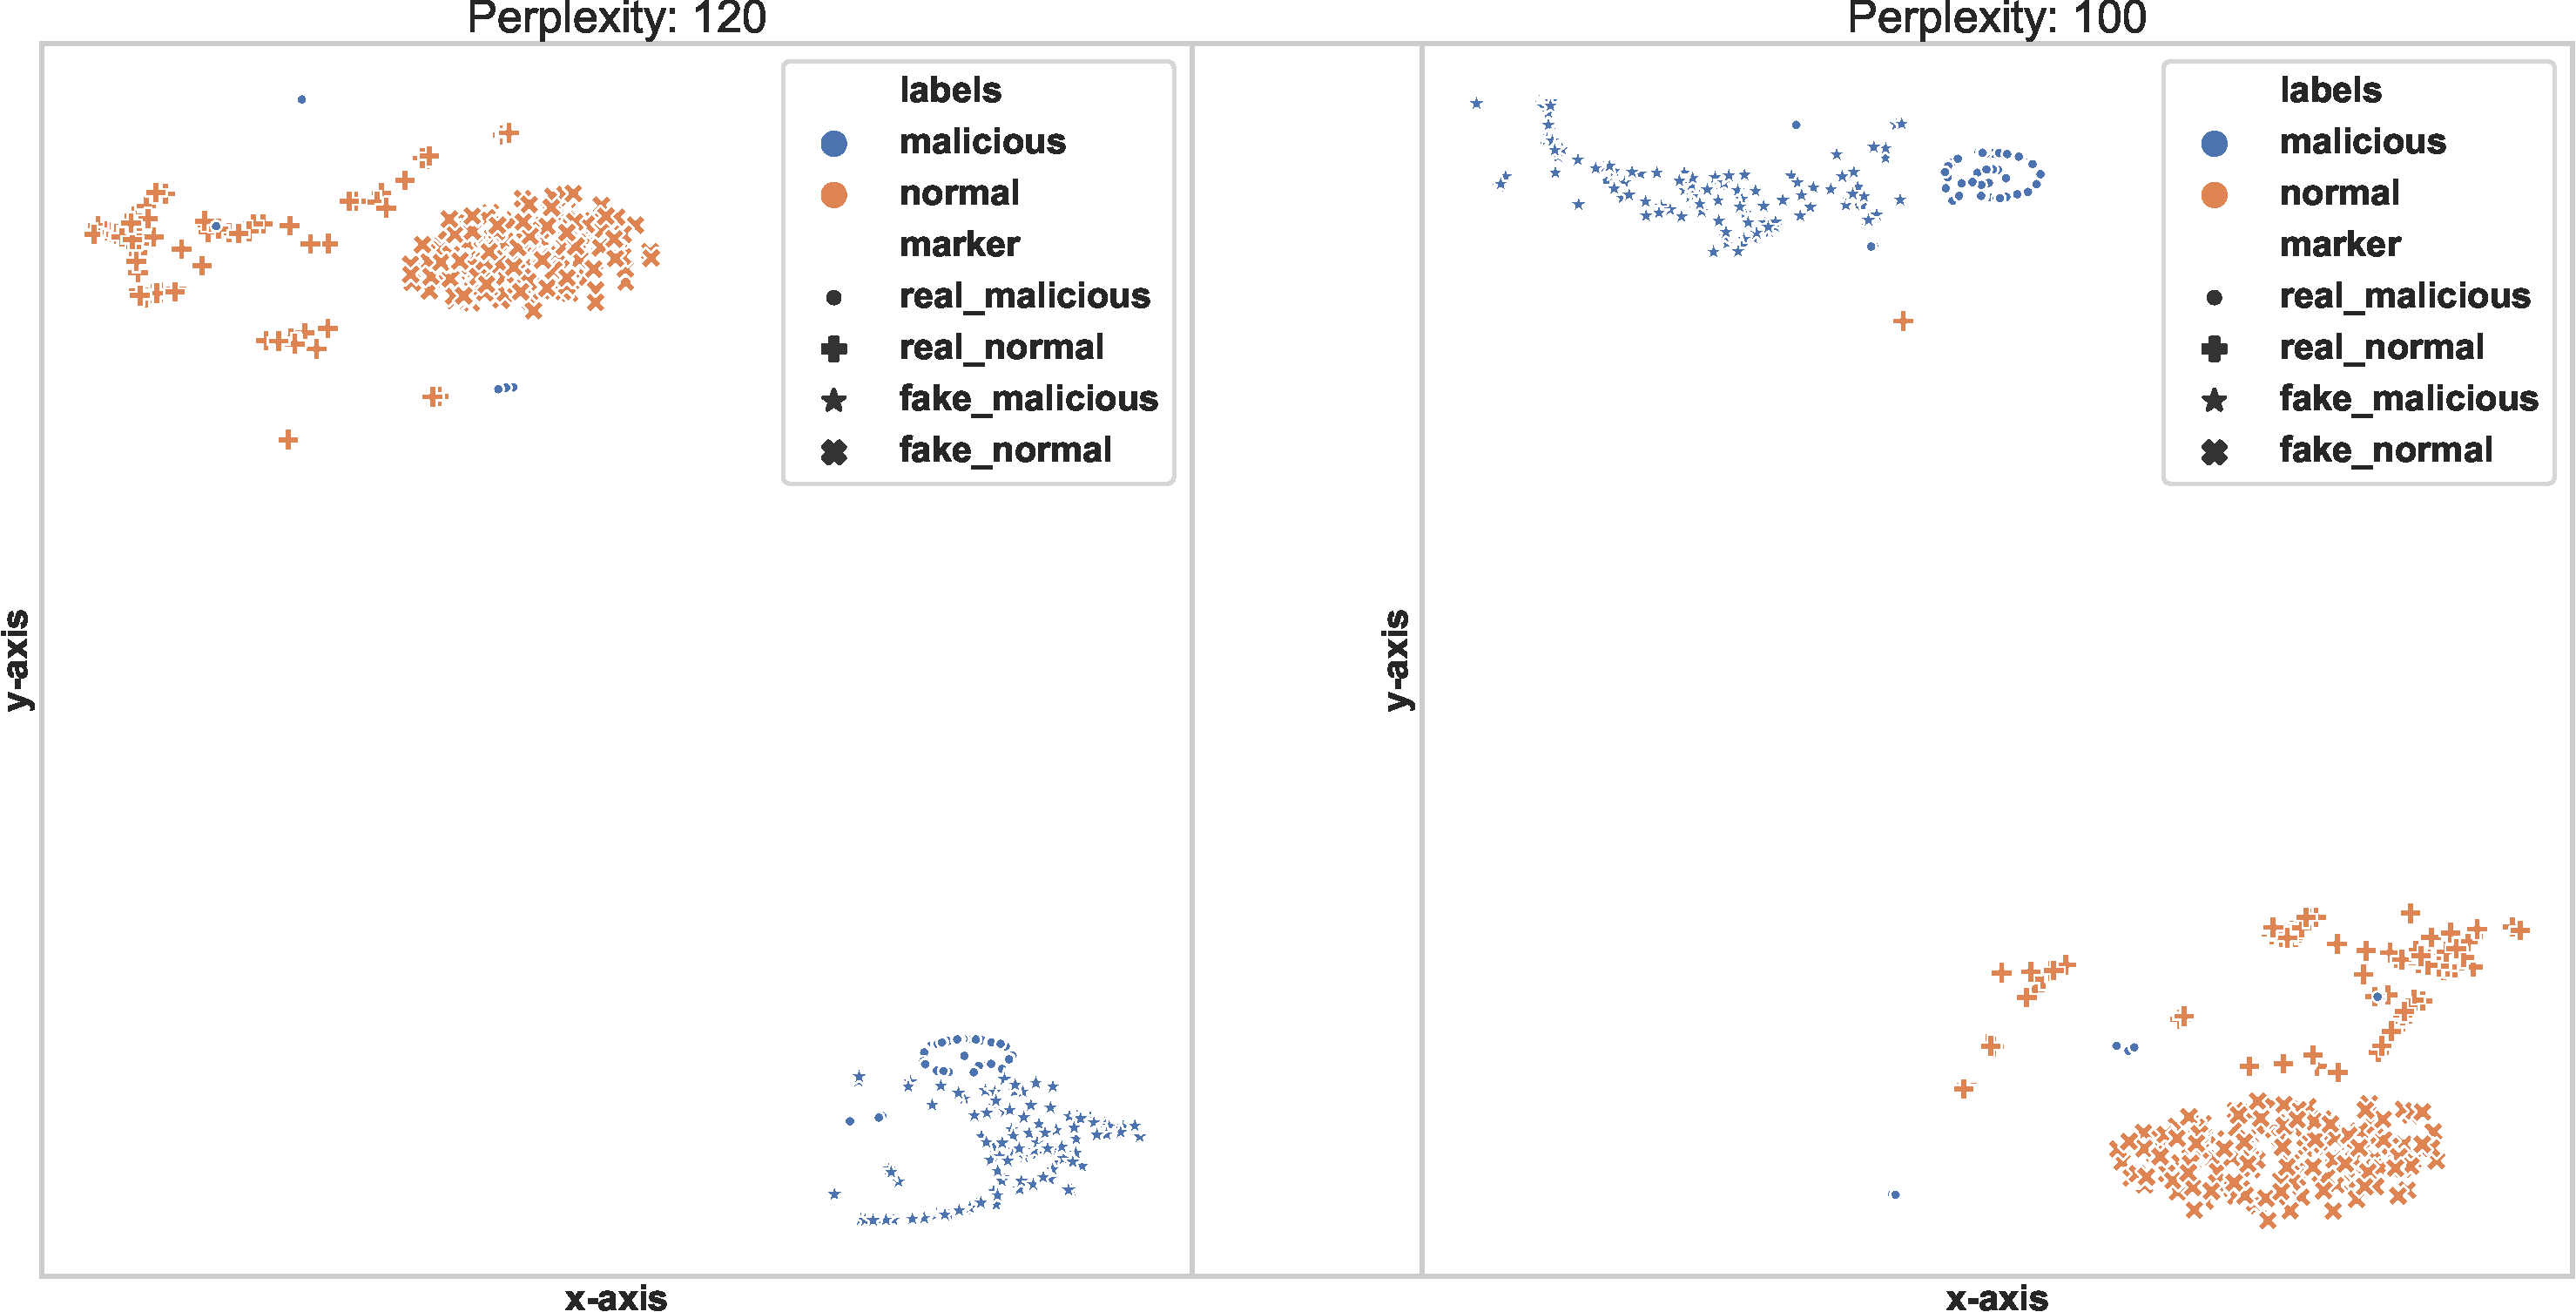
\includegraphics[width=\textwidth,keepaspectratio]{kdd-trained}
	\caption{After Training (KDD99): Binary Class CGAN creates Distinct Clusters for the Malicious and Normal Profiles }
	\label{fig:kdd-trained}
\end{figure*}
\section{Experiments and Results}
\label{sec:experiments}
We test the \textit{AD-CGAN} on two datasets: the \textit{KDD99} network intrusion dataset and the \textit{Amsterdam Library of Object Images (aloi)} \cite{goldstein2016comparative} anomaly dataset. While the \textit{KDD99} has the normal profile as the minority class, the \textit{aloi} dataset has the anomalous profile as the minority class. Also, the two datasets selected for experiments on the framework comprises of image and network log data, thereby providing a diverse environment for measuring the effectiveness of the framework.

\subsection{aloi Dataset}
\label{subsec:aloi}
In this dataset, there are a total of $ \bm{50000} $ samples with $ \bm{3.04\%} $ of the total sample belonging to the anomalous class. This ALOI dataset has $ \bm{27} $ multivariate features. With just $ \bm{1508} $ anomalous samples out of the $ \bm{50000} $ samples, it is difficult to train a model with this dataset without overfitting on the majority class. And since detection of the anomalous samples is more critical than detecting the normal profile, we will adopt the multi-stage process of data augmentation with the \textit{single class CGAN} of Fig. \ref{fig:ad-cgan}. 
\subsubsection{ALOI Single Class CGAN Results}
\label{subsub:aloiscgresults}
As highlighted in Section \ref{subsub:scgan}, the aim of the \textit{single class CGAN} is to understand the profile of the data being trained such that when the \textit{fake} and the \textit{real} samples are subjected to the embedding algorithm, the result should be a single cluster which confirms how the single class CGAN has been able to understand the underlying distribution of the real samples. To measure the performance of the generator, we take snapshots of the model at intervals of $ \bm{50} $ epochs during training. Thereafter, we compare the generated quality at each snapshot and the best model becomes our trained generator model. According to \cite{wattenberg2016how}, the \textit{tSNE} algorithm used for the embedding of Section \ref{subsub:tsne} has a hyperparameter called \textit{perplexity}\footnote{Perplexity is a parameter used to determine the number of close neighbors each point has.}, therefore, we generate the results under different perplexities to measure the stability of the model under varying perplexities. \par 
In Fig. \ref{fig:aloi-a-untrained}, the \textit{fake} and \textit{real} samples show two distinct clusters under different perplexities before we train the generator. After we are done training the generator, we can see that the generator is able to decipher the underlying distribution of the \textit{real} samples as seen in Fig. \ref{fig:aloi-a-trained} where the \textit{real} and \textit{fake} samples form one cluster. The ability of the single class CGAN to generate samples which are indistinguishable from the real samples confirms one of our hypothesis that we can use the generator to \textit{augment the minority class data samples} and train the \textit{binary class CGAN} with a balanced dataset.
\subsubsection{ALOI Binary Class CGAN}
\label{subsub:aloibcgresults}
The binary class CGAN takes input training data from both the original and augmented samples generated from the single class CGAN with the aim of producing the reverse behavioral expectation of the single class CGAN. As the name suggests, the binary class CGAN aims to understand the underlying distributions of both the malicious and normal data samples in such a way that the \textit{fake} and \textit{real} samples from each class belong to the same cluster when subjected to the embedding algorithm and the decision functions of Section \ref{subsub:detector}. As seen in Fig. \ref{fig:aloi-untrained}, the embedding output before training shows a mixture of the positive and negative class in the same cluster, thereby creating both false positive and false negative situation on both the \textit{real} and \textit{fake} samples. In all our result analysis, we designate the malicious samples as the \textit{positive class}. In Fig. \ref{fig:aloi-trained}, the results of the trained model show how the generator output and real test samples have successfully been separated into their respective classes. Although the snapshots of Fig. \ref{fig:aloi-trained} does not show exactly two clusters as hypothesized, from the position of the \textit{fake normal} and \textit{fake malicious} data, we see that when we compute the centroids using \eqref{eq:centroid}, the closest samples are data points that belong to the same class from the test points. Thereby, confirming our hypothesis that the generator can be used to understand the different latent class distributions. And that an embedding of the \textit{fake} and the \textit{real} samples of each class should produce a single cluster that aims to classify samples from that particular class with a higher precision. Also, since the malicious class is our positive class, we can see from Fig. \ref{fig:aloi-trained} that the malicious class forms a single cluster as hypothesized, and this result reduces the chance of false negative to almost zero as shown in Table \ref{tab:aloi-report} and Fig. \ref{fig:auc-curve-aloi}.
\begin{table*}[!t]
	\renewcommand{\arraystretch}{1}
	\caption{Classification Report of AD-CGAN on the ALOI and KDD Dataset}
	\label{tab:aloi-report}
	\centering
	\begin{tabu} to 0.99\textwidth {|X[c]||X[c]|X[c]|X[c]|X[c]|X[c]|X[c]|}
		\hline
		Dataset & Class & Precision & Recall& F1 Score & No. Test Samples 
		& Accuracy   \\
		\hline
		\multirow{2}{*}{ALOI} & Normal & $ 0.96945  $ & $ 0.98905  $ & $ 0.97915 $& $ 10044 $ & \multirow{2}{*}{$ 0.97885 $} \\
		\cline{2-6}
		& Malicious & $ 0.98872$ & $ 0.96856 $ & $ 0.97854 $ & $ 9956 $&  \\
		\hline
		\hline
		\multirow{2}{*}{KDD} & Normal & $ 0.77749   $ & $ 0.99862  $ & $ 0.87429 $& $ 74886 $ & \multirow{2}{*}{$ 0.85663$} \\
		\cline{2-6}
		& Malicious & $ 0.99809 $ & $ 0.71507 $ & $ 0.83320  $ & $ 75114 $&  \\
		\hline
	\end{tabu}
\end{table*}
In Table \ref{tab:aloi-report}, we show the different classification metric of the \textit{ALOI} dataset alongside the total number of test samples for each class. The malicious class test sample consists of the \textit{real} and \textit{fake} samples from the single class CGAN. The perplexity hyperparameter that we use for this testing is $ \bm{150} $, and we sample $ \bm{500} $ samples of the test data at a time. While the binary class CGAN generates samples during testing, the test report evaluates the performance of the model on the \textit{real} input test samples only. The \textit{fake} samples generated by the binary class CGAN during testing controls the position of the centroids. The authors of \cite{campos2016evaluation} have done a comprehensive evaluation of the performance of different algorithms on the most commonly used anomaly datasets. We compare the results of some algorithms used in \cite{campos2016evaluation} on the ALOI dataset to the results of \textit{AD-CGAN} in Table \ref{tab:aloi-comparison}. Since we are using the original dataset with $ \bm{466} $ duplicates of the normal samples, we will be comparing with \textit{clustering} algorithms results on the \textit{normalized, duplicate} results of the ALOI dataset in \cite{campos2016evaluation}. Also, \cite{campos2016evaluation} did evaluation using different hyperparameters on the same algorithm but we report only the one with the highest receiver operating characteristics area under the curve (ROC AUC) value.
\begin{table*}[!t]
	\renewcommand{\arraystretch}{1}
	\caption{Comparison Report of Algorithms on the ALOI and KDD Dataset}
	\label{tab:aloi-comparison}
	\centering
	\begin{tabu} to 0.99\textwidth {|X[c]||X[c]|X[c]|X[c]|X[c]|X[c]|}
		\hline
		\textbf{Dataset}&\textbf{Algorithm} & \textbf{k (nearest neighbor)} & \textbf{Precision} & \textbf{F-1 Score} & \textbf{ROC AUC Score} \\
		\hline
	 	\multirow{11}{*}{ALOI}&\textbf{KNN} & $\bm{1} $ & $ 0.13019	 $ & $ 0.17982 $ & $0.74141$ \\
		\cline{2-6}
		&\textbf{KNNW} & $ \bm{1}$ & $ 0.14090 $ & $ 0.18164 $ & $ 0.74862 $ \\
		\cline{2-6}
		&\textbf{LOF} & $ \bm{9}$ & $ 0.11933 $ & $ 0.19791 $ & $ 0.78437 $ \\
		\cline{2-6}
		&\textbf{SimplifiedLOF} & $ \bm{9}$ & $ 0.13114	 $ & $ 0.21236 $ & $ 0.79755 $ \\
		\cline{2-6}
		&\textbf{LoOP} & $ \bm{12}$ & $ 0.14852$ & $ 0.23272 $ & $ 0.80243 $ \\
		\cline{2-6}
		&\textbf{ODIN} & $ \bm{12}$ & $0.15644	 $ & $ 0.24430 $ & $ 0.80608 $ \\
		\cline{2-6}
		&\textbf{KDEOS} & $ \bm{98}$ & $0.09264 $ & $ 0.15412 $ & $ 0.77409 $ \\
		\cline{2-6}
		&\textbf{LDF} & $ \bm{9}$ & $0.08717 $ & $0.14766 $ & $ 0.74790 $ \\
		\cline{2-6}
		&\textbf{INFLO} & $ \bm{9}$ & $0.13931$ & $ 0.22596 $ & $ 0.80020 $ \\
		\cline{2-6}
		&\textbf{COF} & $ \bm{13}$ & $ 0.14095	 $ & $ 0.21083 $ & $ 0.80353$ \\
		\cline{2-6}
		&\textbf{AD-CGAN} & N/A & $ \bm{0.97909}$ & $ \bm{0.97885} $ & $ \bm{0.9832} $ \\
		\hline
		\hline
		\multirow{11}{*}{KDD}&	\textbf{KNN} & $\bm{85} $ & $ 0.36786 $ & $ 0.48159 $ & $\bm{0.98982}$ \\
		\cline{2-6}
		&\textbf{KNNW} & $ \bm{100}$ & $ 0.11989 $ & $ 0.23577 $ & $ 0.98273 $ \\
		\cline{2-6}
		&\textbf{LOF} & $ \bm{100}$ & $ 0.01091 $ & $ 0.03139 $ & $ 0.82330 $ \\
		\cline{2-6}
		&\textbf{SimplifiedLOF} & $ \bm{34}$ & $ 0.00966 $ & $ 0.04012 $ & $ 0.62814 $ \\
		\cline{2-6}
		&\textbf{LoOP} & $ \bm{34}$ & $ 0.01445 $ & $ 0.06088 $ & $ 0.68726 $ \\
		\cline{2-6}
		&\textbf{ODIN} & $ \bm{100}$ & $0.01327 $ & $ 0.04944 $ & $ 0.78924 $ \\
		\cline{2-6}
		&\textbf{KDEOS} & $ \bm{50}$ & $0.01130 $ & $ 0.05336 $ & $ 0.61999 $ \\
		\cline{2-6}
		&\textbf{LDF} & $ \bm{87}$ & $0.02674 $ & $ 0.06834	 $ & $ 0.88959 $ \\
		\cline{2-6}
		&\textbf{INFLO} & $ \bm{25}$ & $0.01095 $ & $ 0.05044 $ & $ 0.64848 $ \\
		\cline{2-6}
		&\textbf{COF} & $ \bm{35}$ & $ 0.01278 $ & $ 0.06275 $ & $ 0.61605 $ \\
		\cline{2-6}
		&\textbf{AD-CGAN} & N/A & $ \bm{0.88796}$ & $ \bm{0.85372} $ & $ 0.89300 $ \\
		\hline
	\end{tabu}
\end{table*}
\subsection{KDD99 Dataset}
\label{subsec:kdd}
Unlike the ALOI dataset of Section \ref{subsec:aloi}, the \textit{KDD99} dataset has more than two categories of data which are broadly classified into \textit{malicious} and \textit{normal} profiles. Since the test data has more categories of anomalies that are not available in the training data, we converted the whole data into two categories by collapsing any non-normal category to a new category called \textit{malicious} profile. This way, AD-CGAN can be tested on any kind of normal or anomalous scenarios that were not available during the training phase. One of the strengths of \textit{AD-CGAN} which we highlight in this test is the ability of the model to train on a small subset of the data and still generalize well on the rest of the test data. Traditional machine learning algorithms train on a larger portion of the data and usually reserve between $ \bm{10\%-20\%} $ of the data for evaluation and testing. However, in the \textit{AD-CGAN} model, we show that we can relax this convention and still achieve great model performance. The model is able to generalize even when trained on a small subset of the data because CGANs have inherent ability to draw knowledge from the \textit{latent} space distribution of the data used for training. \par 
After we binarized the data, the \textit{KDD99} dataset has $ \bm{3925650} $ samples of the malicious profile and $ \bm{972781} $ samples of the normal profile with $ \bm{41} $ multivariate features. Instead of training on the whole dataset, we train on a balanced subset of the data comprising of $ \bm{772781} $ samples from the normal profile and $ \bm{772781} $ from the malicious profile. This training sample represents $ \bm{31.55\%} $ of the whole dataset, and this percentage contrasts with the normal convention of training on larger subsets of the data. We sample the test data from the remaining subsets of the data. \par 
Since our model depends on the perplexity parameter of the embedding layer, we used hyperparamter tuning to determine the optimum perplexity. For our evaluations on KDD99 dataset, we use $ \bm{120} $ as the perplexity parameter, and we sample a batch of $ \bm{300} $ test samples at a time. Therefore, in Fig. \ref{fig:kdd-untrained}, the \textit{real} and \textit{fake} samples of both the normal and malicious profiles form several indistinguishable clusters before we train the model. This figure acts as a baseline for the trained model. Furthermore, in Fig. \ref{fig:kdd-trained}, the \textit{real} and \textit{fake} samples of the normal profile class form a single, distinct cluster while the \textit{real} and \textit{fake} samples of the malicious profile class form a separate, distinct cluster after training the generator. This contrast in the behavior of the generator after training confirms our hypothesis that the CGANs can be used to learn the context of the data, and form the basis for anomaly detection.

\section{Discussion of Results}
\label{sec:results}
In Table \ref{tab:aloi-report}, we show the metrics of the AD-CGAN when tested on the ALOI and the KDD99 dataset. In the ALOI dataset, we sample randomly from both the \textit{augmented data} from the single class CGAN and the original anomalous data. The number of data samples tested is included in Table \ref{tab:aloi-report} and we can see that with $ \bm{20000} $ data samples tested, the accuracy of the model and other metrics show effective detection of malicious samples with almost zero false positives. We attribute the ability of the AD-CGAN to achieve this level of performance on the false positive metric on the inherent nature AD-CGAN to use the latent knowledge of the distribution of the data to reduce the effect of noise during testing. Since the \textit{positive class} is our malicious profile data, the data of Table \ref{tab:aloi-report} confirms the effectiveness of AD-CGAN on the ALOI dataset as it reports high precision and recall on both classes of data. Similarly, in Table \ref{tab:aloi-report}, we report the class-based metrics for the KDD99 dataset as tested on $ \bm{150000} $ samples of the test data. As seen from Table \ref{tab:aloi-report}, for $ \bm{150000} $ samples of the test data, the precision score of the malicious profile achieves one of our objectives of reducing false positives while ensuring that we detect the malicious profiles in the system. This high precision score ensures that while we detect the actual malicious profiles, we do not invest resources to investigate false alarms. And since the positive class is the malicious profile, this high precision at the cost of lower recall is preferable.  \par
Also, in Table \ref{tab:aloi-comparison}, we compare the performance of AD-CGAN on the ALOI dataset with other cluster-based algorithms that have been used on the data. We report only the \textit{normalized, duplicate} and the \textit{normalized, duplicate, 1-of-n encoding} versions of the ALOI and KDD99 dataset experiments respectively from \cite{campos2016evaluation} because we took similar preprocessing steps. We select the \textit{average precision, maximum F-1 score}, and the \textit{ROC AUC} score for comparison because those are the common metrics reported in \cite{campos2016evaluation}. From the results in Table \ref{tab:aloi-comparison} under the ALOI dataset category, AD-CGAN outperforms all the other algorithms in all the metrics reported. 
 Although \cite{campos2016evaluation} trained and tested on a very small subset of the KDD99 dataset of about $ \bm{60839}  $ while we train and test on the full dataset of about $ \bm{4,898,431} $ samples, we compare the performance of AD-CGAN because while some metrics like ROC AUC may vary with sample size and class imbalance, some others like \textit{accuracy, precision, recall} is expected to be stable irrespective of the sample size for a well designed algorithm. Therefore, in Table \ref{tab:aloi-comparison}, we compare the results of other clustering-based algorithms as reported in \cite{campos2016evaluation} to AD-CGAN. While the KNN algorithm has a better ROC AUC score, AD-CGAN outperforms all other algorithms in the average precision and F-1 scores. Since the ROC AUC are a function of sample size and class balance, we posit that the high ROC AUC score of KNN on KDD99 dataset is because of the small sample of data that it was trained and tested on. \par 
In Fig. \ref{fig:auc-curve-aloi}, we plot the ROC curves for the ALOI and KDD99 datasets with the malicious profiles designated as the positive class. The curves show that AD-CGAN has high precision for the malicious profiles of both data but the confidence in the KDD99 dataset is lower than in that of the ALOI dataset. This behavior is expected because the KDD99 test dataset has some anomalous types that are not present in the training sample. Therefore, even though AD-CGAN is able to detect these profiles with high precision, the true positive rate will not be the same when compared with dataset that has similar profile types in both the test and training samples. 

\section{Conclusion and Future Works}
In this research work, we introduce AD-CGAN, a CGANs-based anomaly detector for both balanced and imbalanced data. With the multi-stage transfer learning knowledge from the CGANs, we are able to eliminate the inherent bias introduced by class imbalance in data. We compare AD-CGAN performance with other cluster-based algorithms and the report show that AD-CGAN returns superior scores in almost all fronts. One of our objectives is to design an anomaly detector that reduces false positives while improving malicious profile detection accuracy, and from the metrics reported in this work, AD-CGAN achieves this with high precision that ensures that false positive is almost zero. Also, even though our sampling frequency is $ \bm{500} $ and $ \bm{300} $ samples respectively for the ALOI and KDD99 datasets respectively, AD-CGAN can operate in as little as $ \bm{> 20} $ samples during testing. This provides high flexibility for users to tune the algorithm according to their desired frequency of operation depending on the kind of application being monitored.\par 
One limitation of the AD-CGAN algorithm we discovered is that the single class CGAN can not train on data in which the minority class data is only a handful of samples ($ \bm{<900} $), therefore, in our future research endeavors, we will be looking to improve AD-CGAN to be able to handle this set of data. 
\label{sec:conclusion}
\bibliographystyle{IEEETran}
\bibliography{access}

\begin{IEEEbiography}[{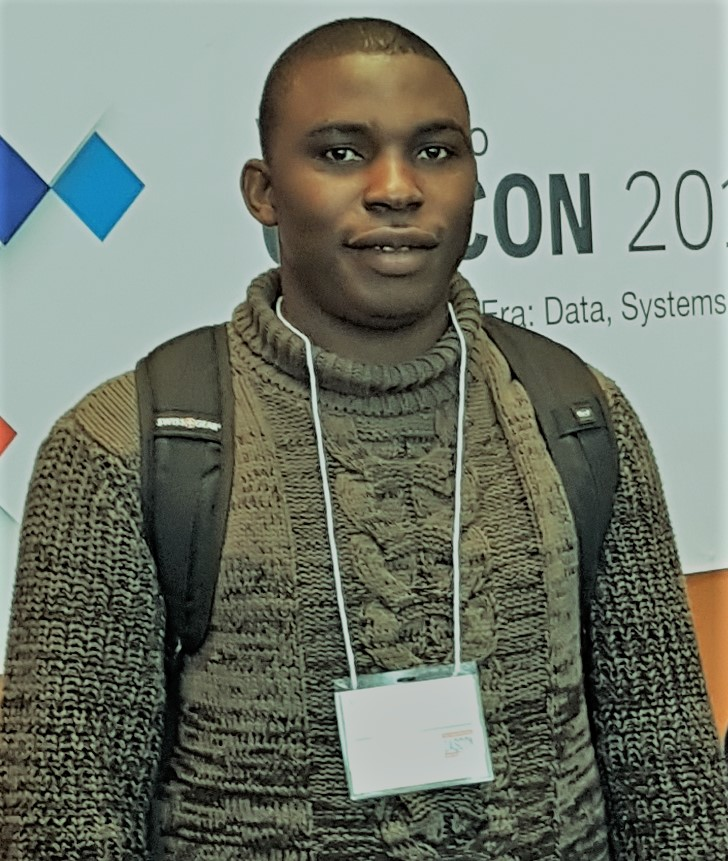
\includegraphics[width=1in,height=1.25in,clip,keepaspectratio]
		{tarbo-image}}]{Okwudili M. Ezeme}
	is a Ph.D. candidate in the  Department of Electrical, Computer and Software 
	Engineering, Ontario Tech University, Oshawa,  
	Ontario, Canada. He received the M.Sc. degree from the Department of 
	Electrical and Computer Engineering, University of Toronto (UofT), Ontario, 
	Canada in 2015, and the  B.Engr. degree in Electronics Engineering 
	from the University of Nigeria, Nsukka (UNN), Nigeria in 2010. His current 
	research interests include deep recurrent neural networks, time-series data 
	processing,  generative adversarial networks and distributed processing in Internet of Things (IoT) devices.
\end{IEEEbiography}

\begin{IEEEbiography}[{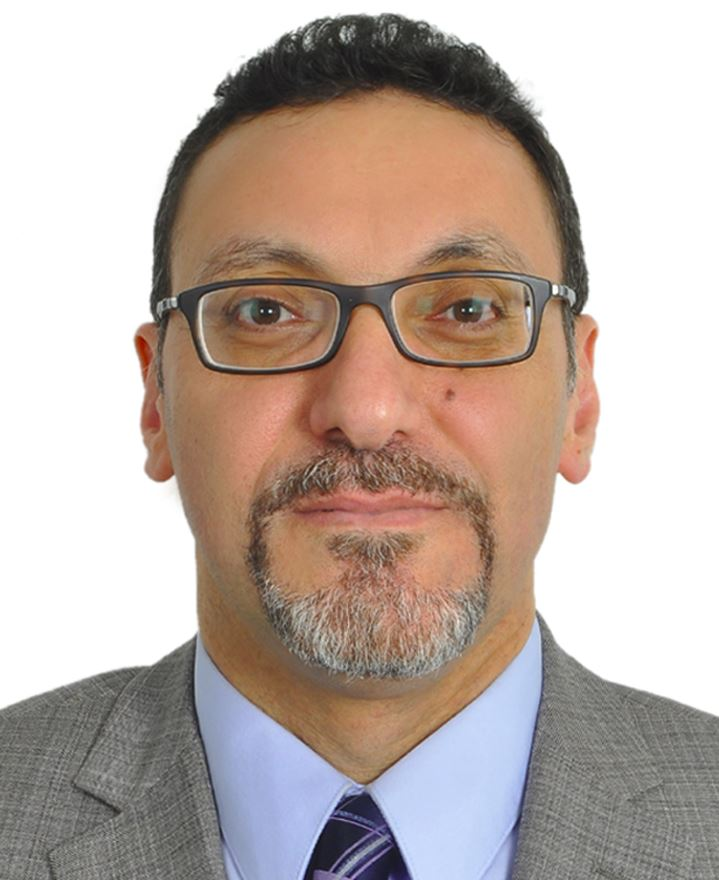
\includegraphics[width=1in,height=1.25in,clip,keepaspectratio]{qusay-image}}]{Qusay
		H. Mahmoud}
	is a Professor of Software Engineering in the Department of Electrical, Computer, and Software Engineering at Ontario Tech University in Oshawa, Canada. He was the Founding Chair of the Department, and more recently he has served as Associate Dean of the Faculty of Engineering and Applied Science at the same university. His research interests include intelligent software systems and cybersecurity.
\end{IEEEbiography}

\begin{IEEEbiography}[{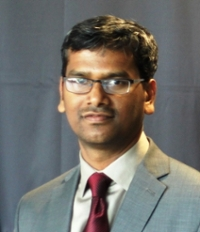
\includegraphics[width=1in,height=1.25in,clip,keepaspectratio]{azim-image}}]{Dr.
		Akramul Azim}
	is an assistant professor in the Department of Electrical, Computer and 
	Software Engineering and head of the real-time embedded software (RTEMSOFT) 
	research group at Ontario Tech University, 
	Oshawa, Ontario, Canada. His research interests include real-time systems, 
	embedded software, software verification and validation, safety-critical 
	software and intelligent transportation systems. He is a Professional Engineer 
	in Ontario and a senior member of IEEE.
\end{IEEEbiography}


\EOD

\end{document}
